\makepart{AI 101: From Fundamentals to Deep Learning}

\section{Introduction to Artificial Intelligence}
\subsection{Deep Learning in the AI family}


\begin{frame}{}
	\begin{columns}[T,onlytextwidth]
		\column{0.4\textwidth}
		In general, among all the class of AI algorithms, we make the difference between 3 sub-categories :
		\begin{itemize}
			\item \alert{Artificial Intelligence} : human designed program and...
			\item \alert{Machine Learning} : human designed features with learned mapping such as Support Vector Machine, Kernels methods, Logistic Regression and ...
			\item \alert{Deep Learning: } Learned features with learned mapping such as Multilayer Perceptron, Convolutional Networks, ...
		\end{itemize}

		\column{0.6\textwidth}
		\begin{figure}
			\centering
			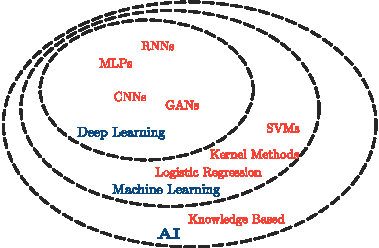
\includegraphics[width=0.9\textwidth]{figures/IAMLDL.pdf}
			\caption{Subsets of Artificial Intelligence}
		\end{figure}
	\end{columns}
\end{frame}

\begin{frame}{}

	\begin{columns}[T,onlytextwidth]
		\column{0.7\textwidth}
		In the field of Artificial Intelligence, the fundamental objective is to find a function $f$ that can perform a desired task. This function can either be set by a human or can be learned through training. \newline

		For example, in the context of a binary classification task, the goal is to determine $f(x)$ such that $f(x) = 0$ when the label of $x$ is 0 and $f(x) = 1$ when its label is 1. The choice of AI model impacts the expressivity of the function $f$. \newline

		For example, a logistic regression model uses a linear function to make decisions, where $f(x) = \mathrm{sgn}(Ax+b)$. The expressivity of the model can be increased by using more complex functions, such as polynomials or radial basis functions.
		\column{0.25\textwidth}
		\begin{figure}
			\centering
			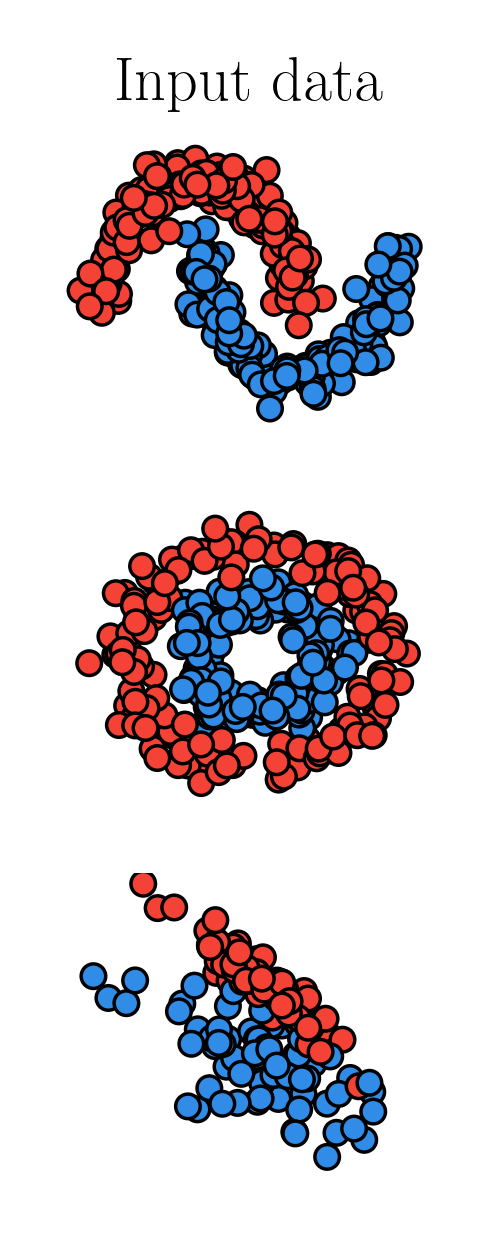
\includegraphics[width=0.7\textwidth]{figures/2Ddata.png}
		\end{figure}
	\end{columns}

\end{frame}

\begin{frame}{}{Classification task}
	\begin{figure}
		\centering
		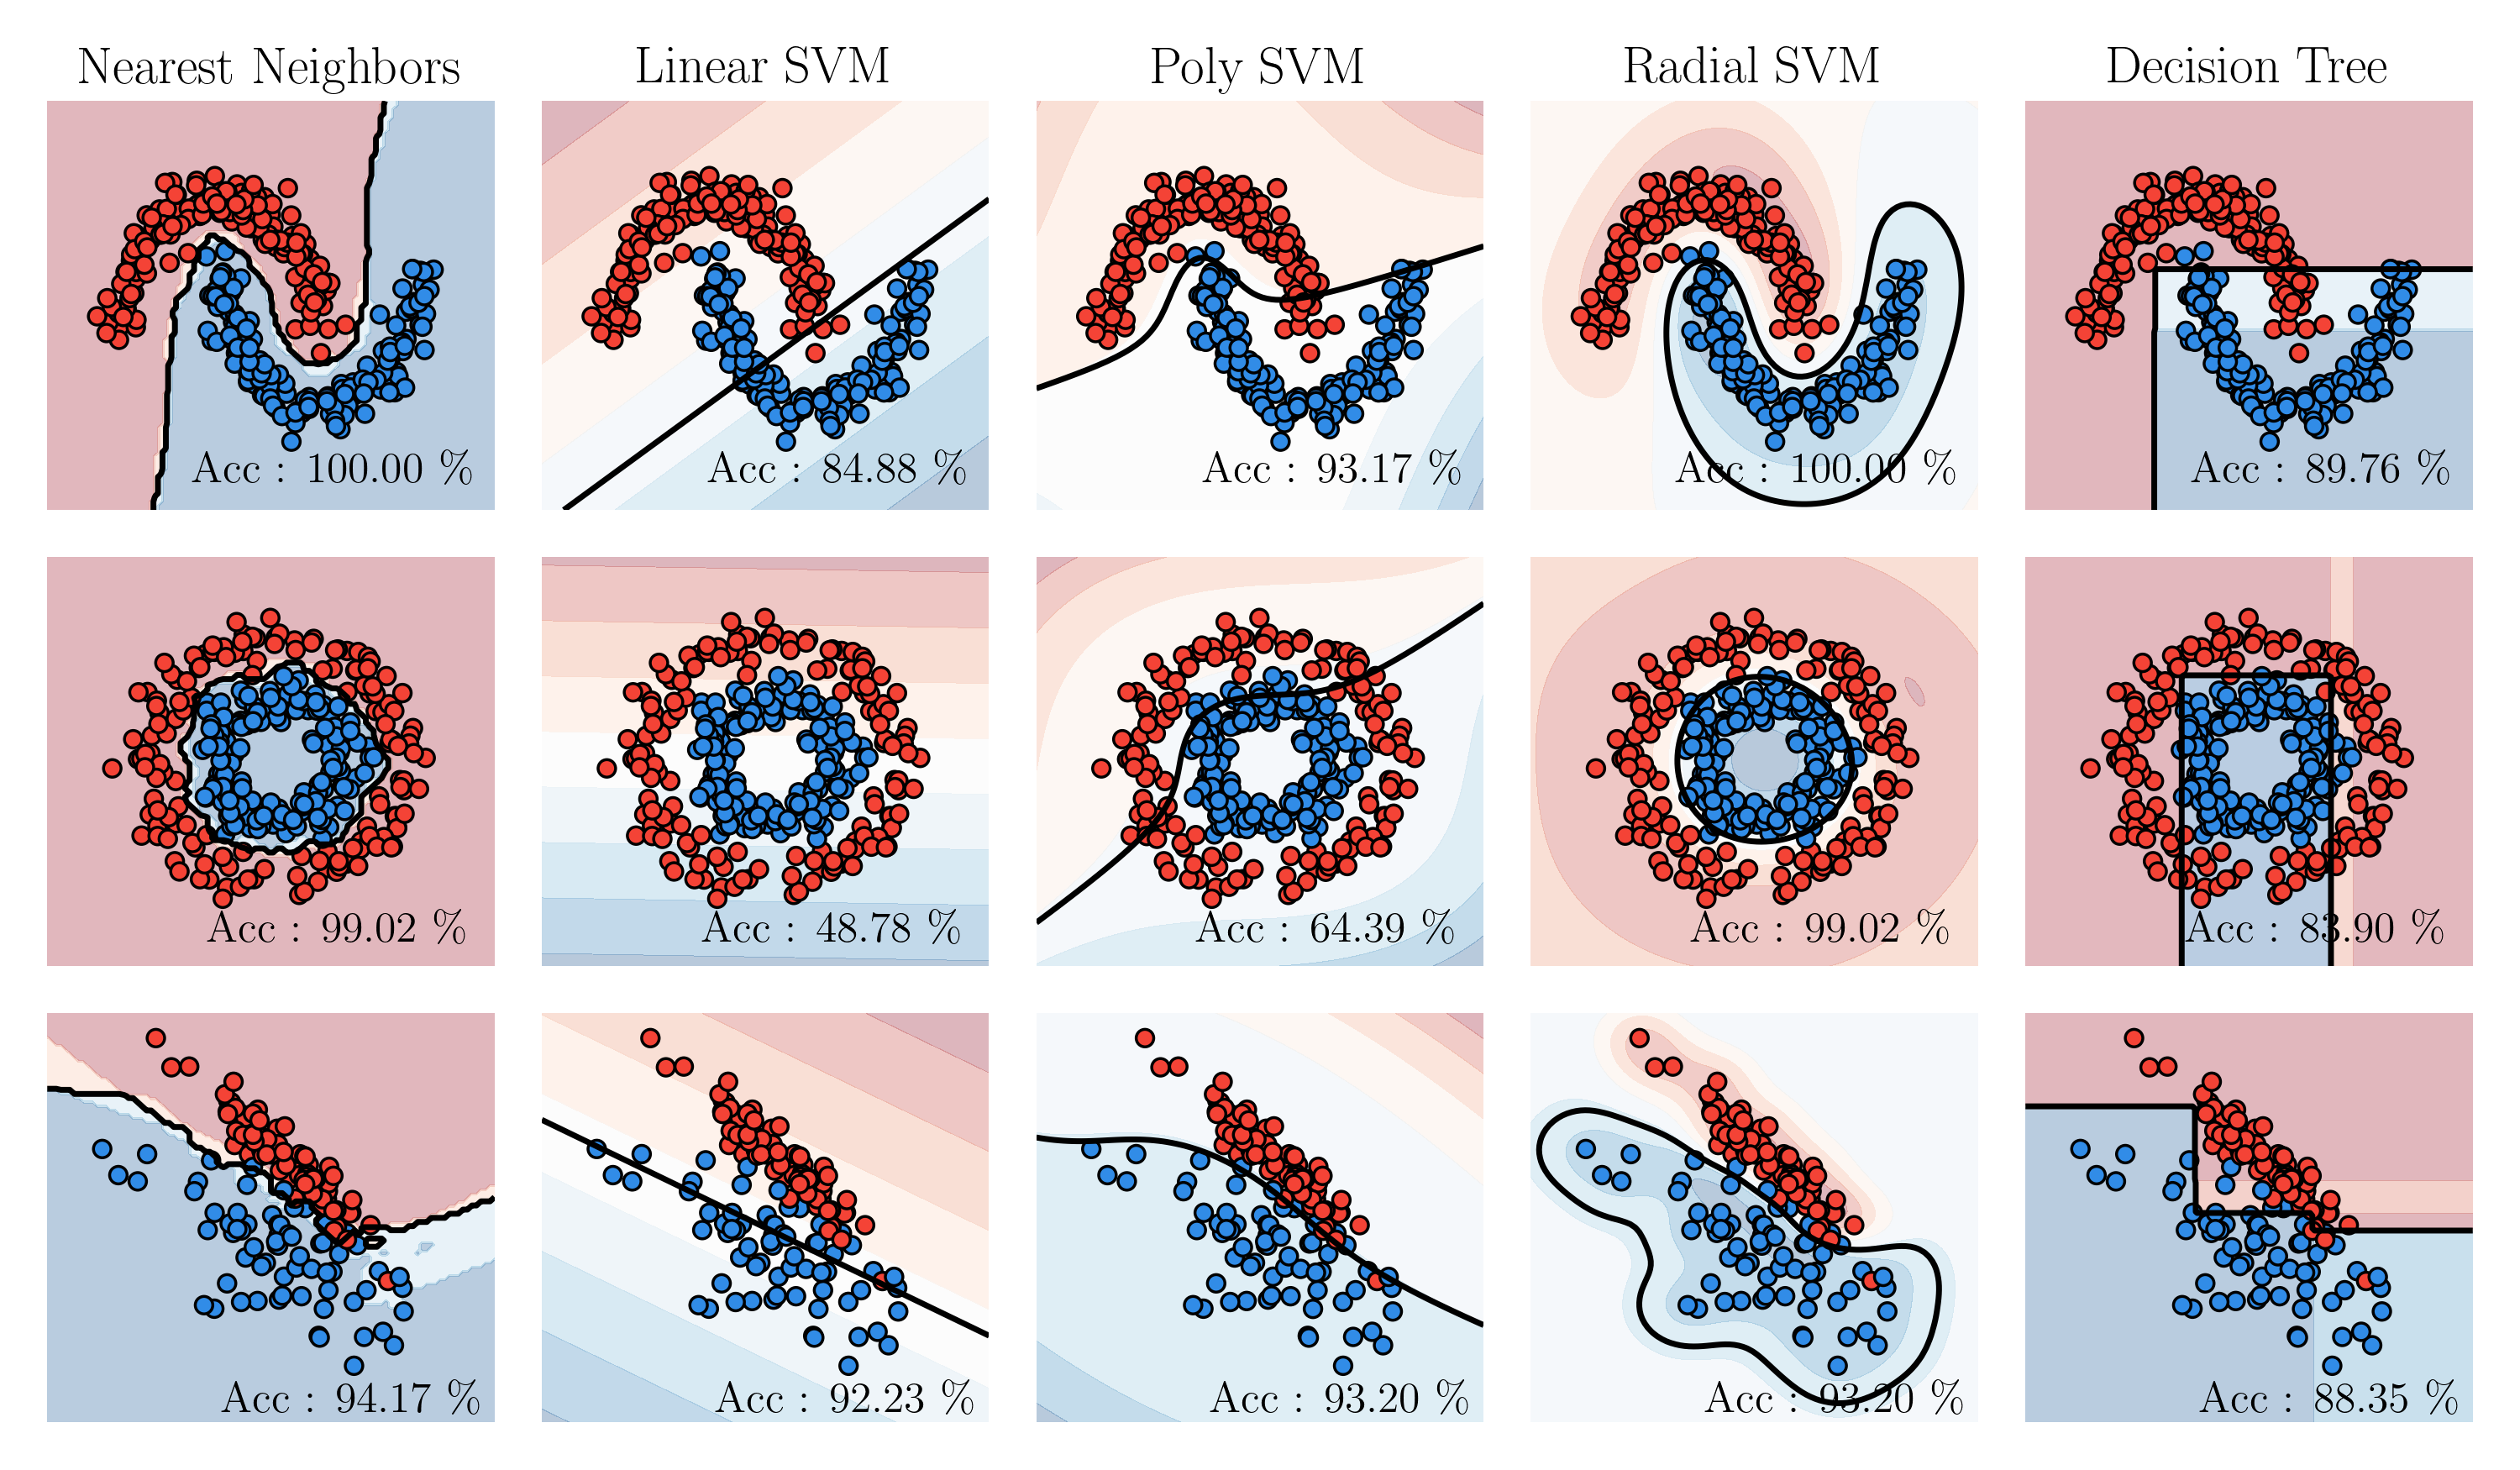
\includegraphics[width=0.8\textwidth]{figures/2Dmodels.png}
		\caption{2D classification for different AI models.}
	\end{figure}
\end{frame}

\begin{frame}{}{The Universal Approximation Theorem}
	The Universal Approximation Theorem is a fundamental result in the field of artificial neural networks. It states that a deep learning model can approximate any function.
	\begin{theorem}[Universal Approximation Theorem]
		Let $\mathcal{ X}\subset \mathbb{R}^d$ be compact, $ \mathcal{Y}\subset \mathbb{R}^m$, $f : \cal X \rightarrow \cal Y$  be a continuous function and $\sigma : \mathbb{R} \rightarrow \mathbb{R}$ be a continuous real function.\newline
		Then $\sigma$ is not polynomial if and only if for every $\epsilon >0$, there exist $k\in \mathbb{N}$, $A\in \mathbb{R}^{k\times d}$, $b\in \mathbb{R}^{k}$ and $C\in \mathbb{R}^{m\times k}$ such that
		$$
			\sup_{x\in \cal X} \Vert f(x)-g(x)\Vert \leq \epsilon
		$$
		where $g(x) = C \times \sigma(Ax+b)$.
	\end{theorem}
\end{frame}

\begin{frame}{}{Classification task}
	\begin{figure}
		\centering
		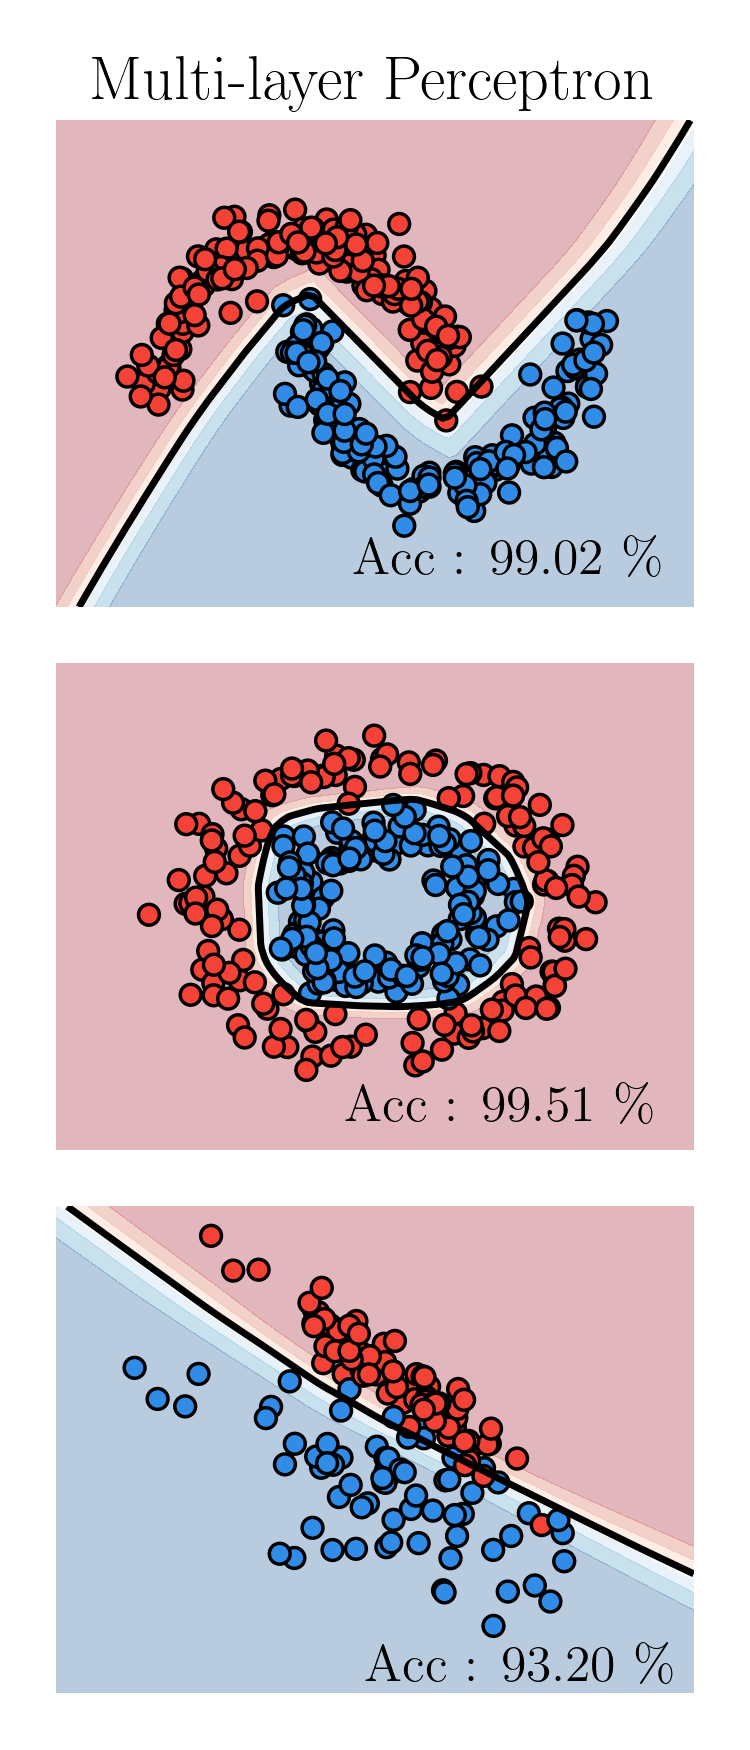
\includegraphics[width=0.2\textwidth]{figures/2DMLP.png}
		\caption{2D classification for small Neural Network.}
	\end{figure}
\end{frame}

\subsection{Representation Learning}


\begin{frame}
	How does deep learning work in practice ?
	\newline

	Deep learning is a subset of representation learning that uses deep neural networks to learn meaningful representations of data. In deep learning, representations are learned through a hierarchy of nonlinear transformations, where each layer of the network builds upon the previous one to extract increasingly abstract and higher-level features from the input data.
	\begin{figure}
		\centering
		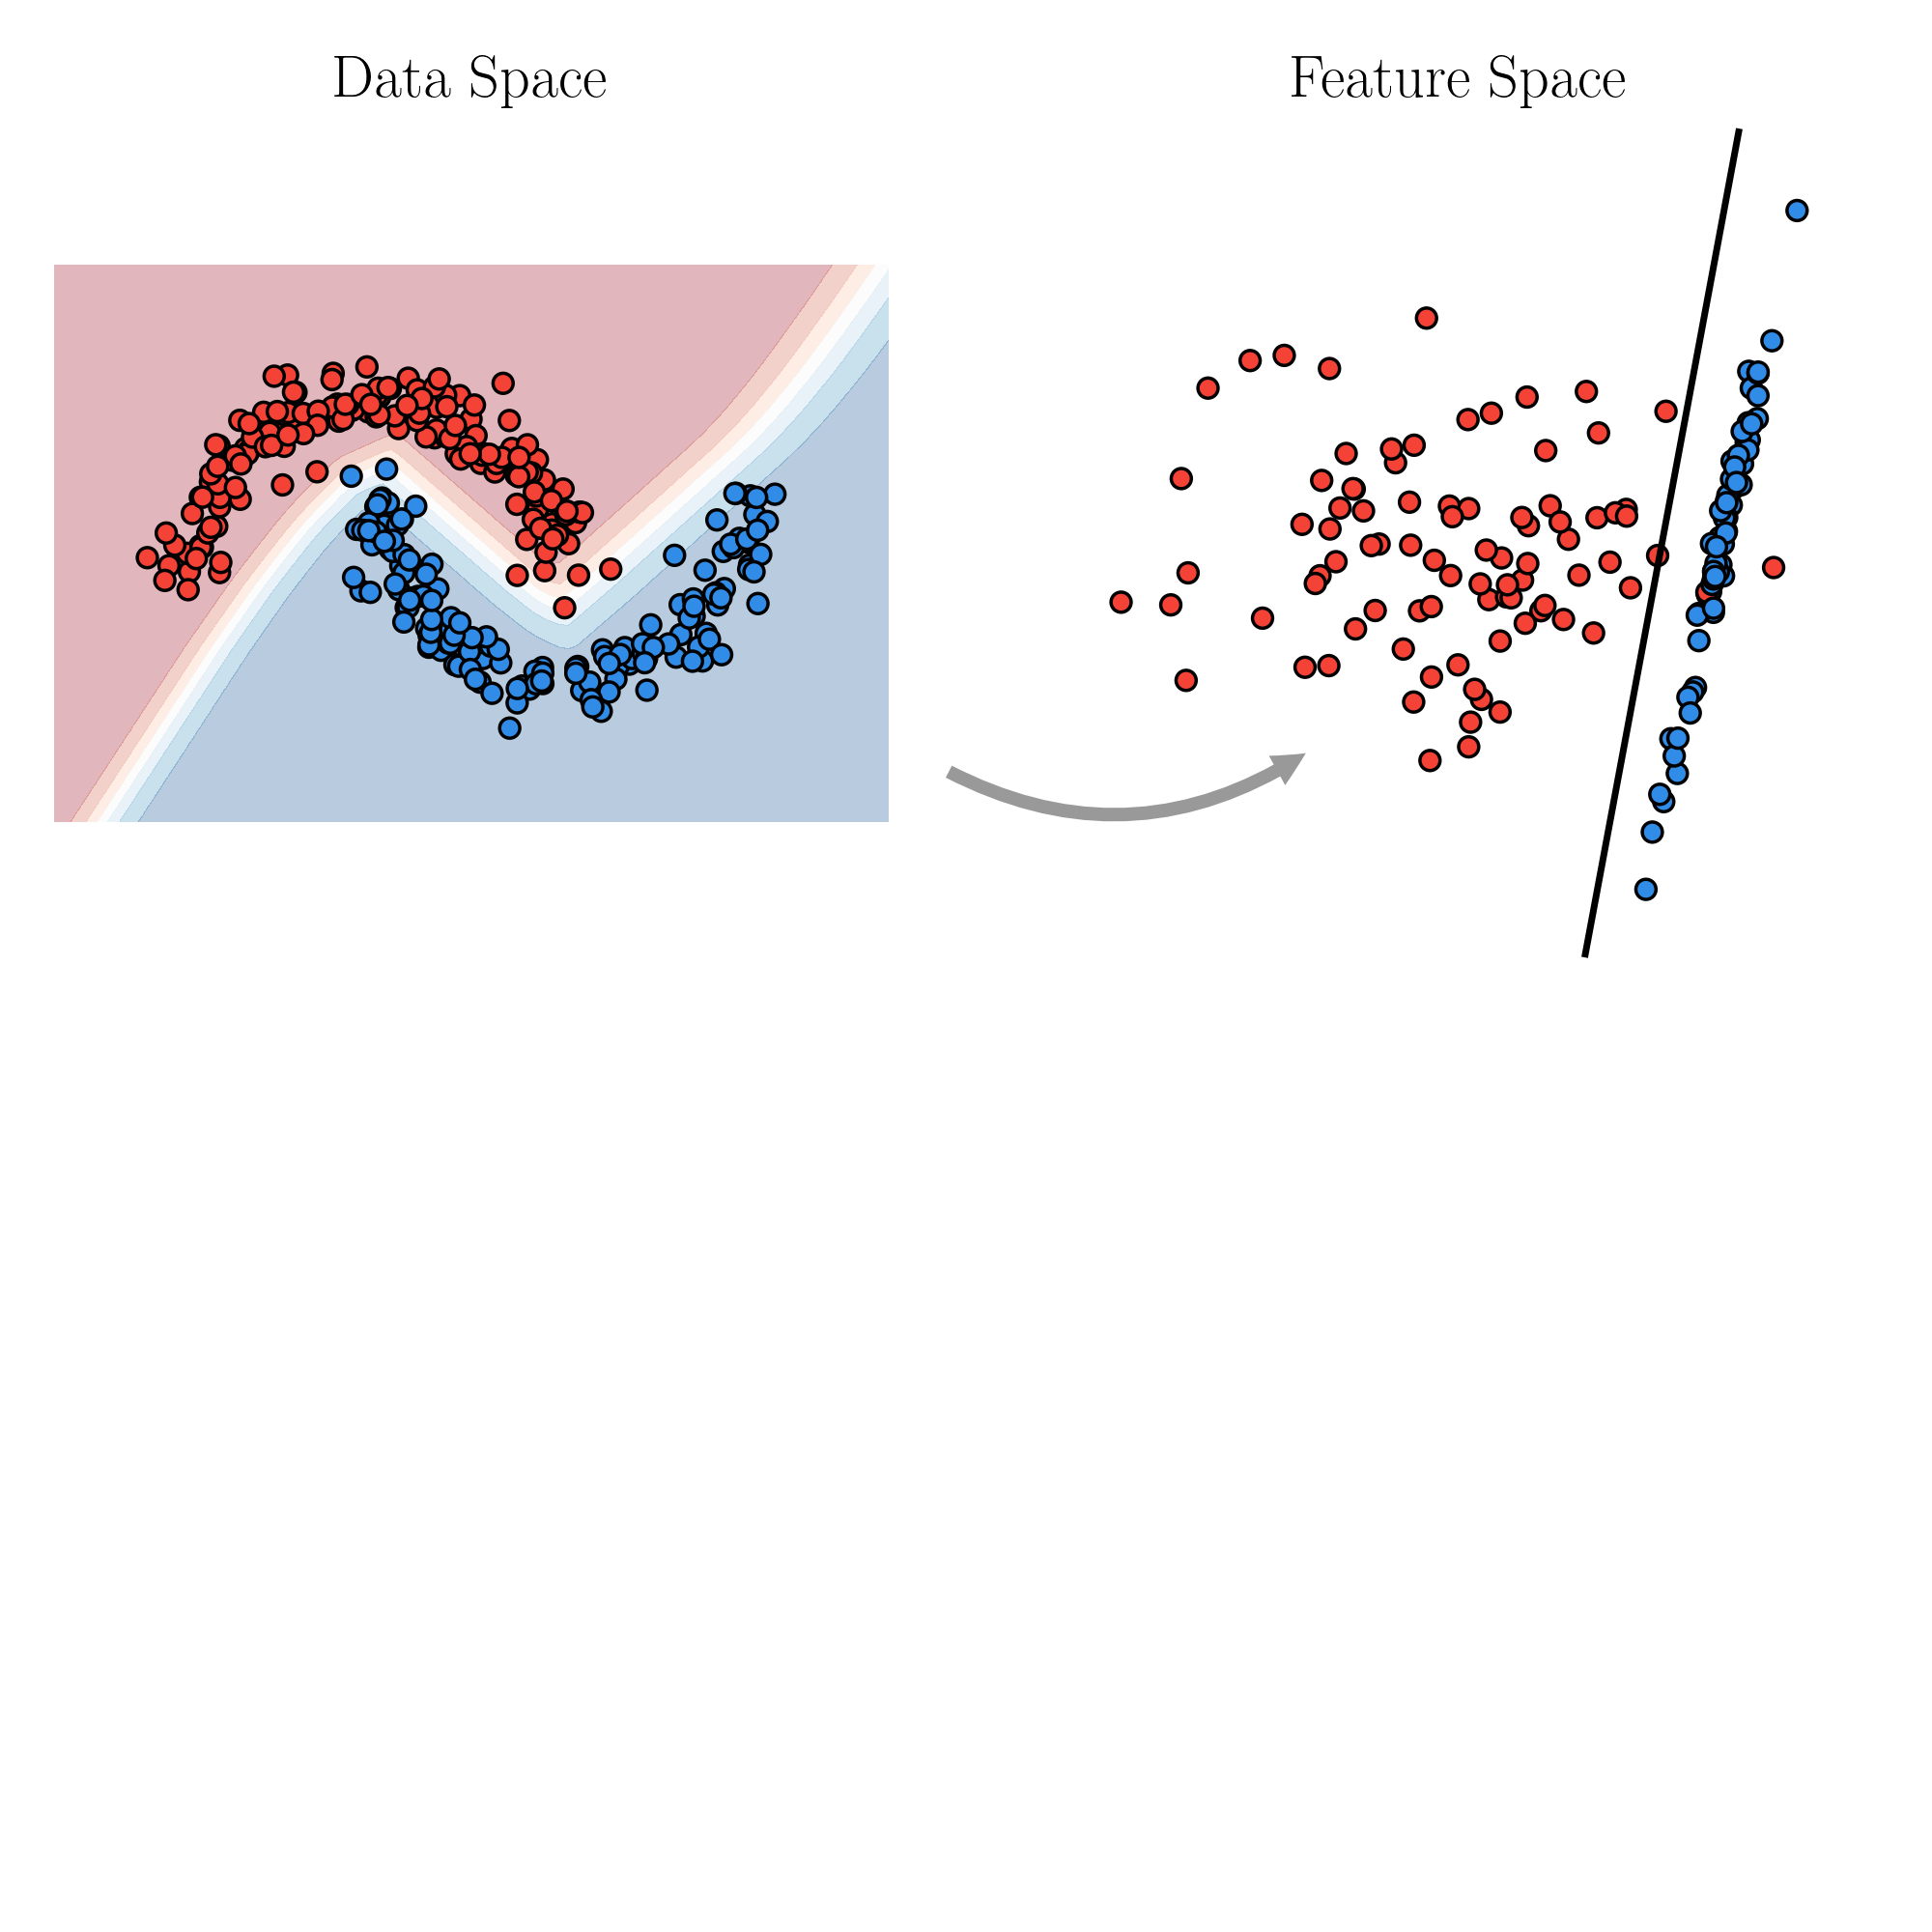
\includegraphics[width=0.6\textwidth]{figures/2DFeature.png}
	\end{figure}
\end{frame}

\begin{frame}{}{Example of Representation Learning}

	\begin{columns}[T,onlytextwidth]
		\column{0.7\textwidth}
		Consider the task of recognizing objects in images. A traditional approach would be to hand-engineer features such as edge detectors and color histograms that can be fed into a classifier. \\
		However, with deep learning representation learning, the model learns to automatically discover these features from the data. The network might start by learning simple features such as edges and color blobs in the first layer, then build upon these to learn more complex features such as parts of objects in subsequent layers, until finally, the final layer outputs a probability distribution over classes of objects. \\

		In this way, deep learning of representation enables the model to automatically learn a rich and meaningful representation of the data, without the need for manual feature engineering.
		\column{0.3\textwidth}
		\begin{figure}
			\centering
			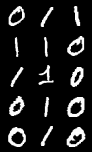
\includegraphics[width=0.7\textwidth]{figures/MNIST.png}
			\caption{MNIST}
		\end{figure}
	\end{columns}
\end{frame}

\begin{frame}{}{Example of Representation Learning}
	\begin{columns}[c,onlytextwidth]
		\column{0.25\textwidth}
		\begin{figure}
			\centering
			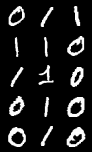
\includegraphics[width=0.7\textwidth]{figures/MNIST.png}
			\caption{MNIST : Layer 0}
		\end{figure}
		\column{0.25\textwidth}
		\begin{figure}
			\centering
			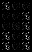
\includegraphics[width=0.7\textwidth]{figures/MNIST_l1.png}
			\caption{MNIST : Layer 1}
		\end{figure}
		\column{0.5\textwidth}
		\begin{figure}
			\centering
			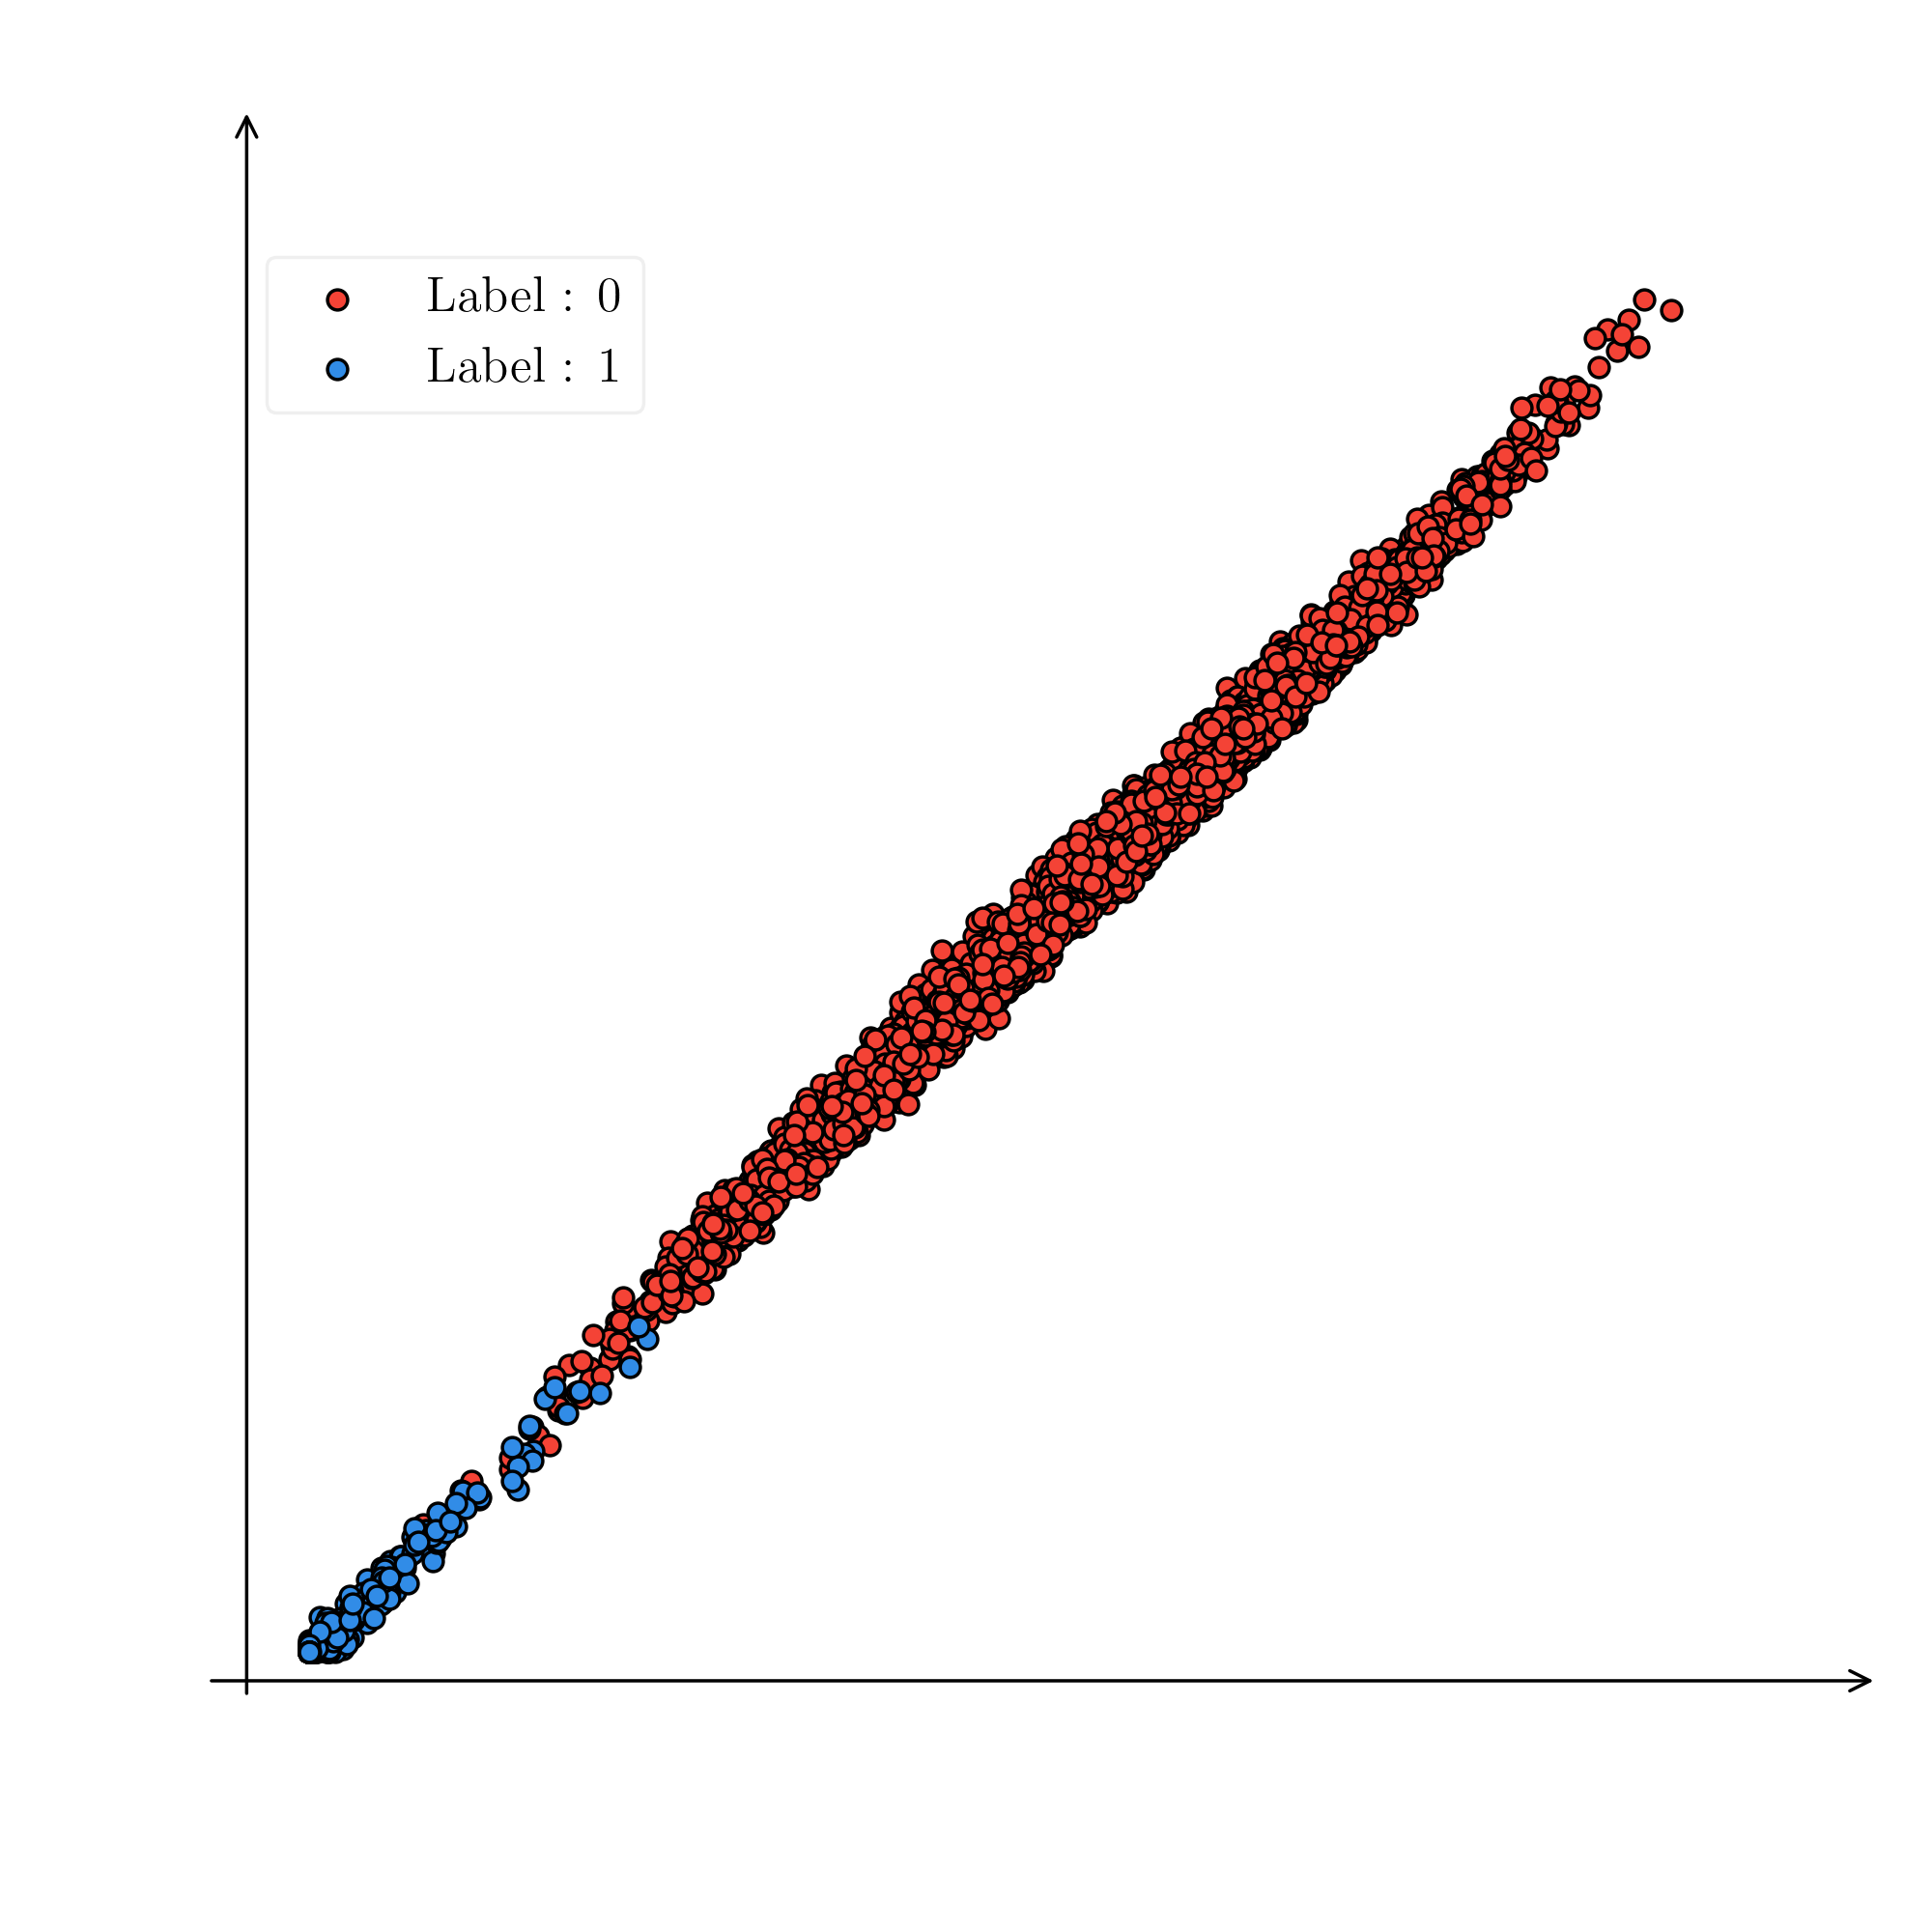
\includegraphics[width=0.9\textwidth]{figures/MNIST_l2.png}
			\caption{MNIST : Layer 2}
		\end{figure}
	\end{columns}
\end{frame}


\begin{frame}{}{Example of Representation Learning}
	\begin{columns}[c,onlytextwidth]
		\column{0.4\textwidth}
		\begin{figure}
			\centering
			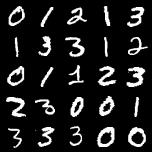
\includegraphics[width=0.7\textwidth]{figures/MNIST_full.png}
			\caption{MNIST : Layer 0}
		\end{figure}
		\column{0.6\textwidth}
		\begin{figure}
			\centering
			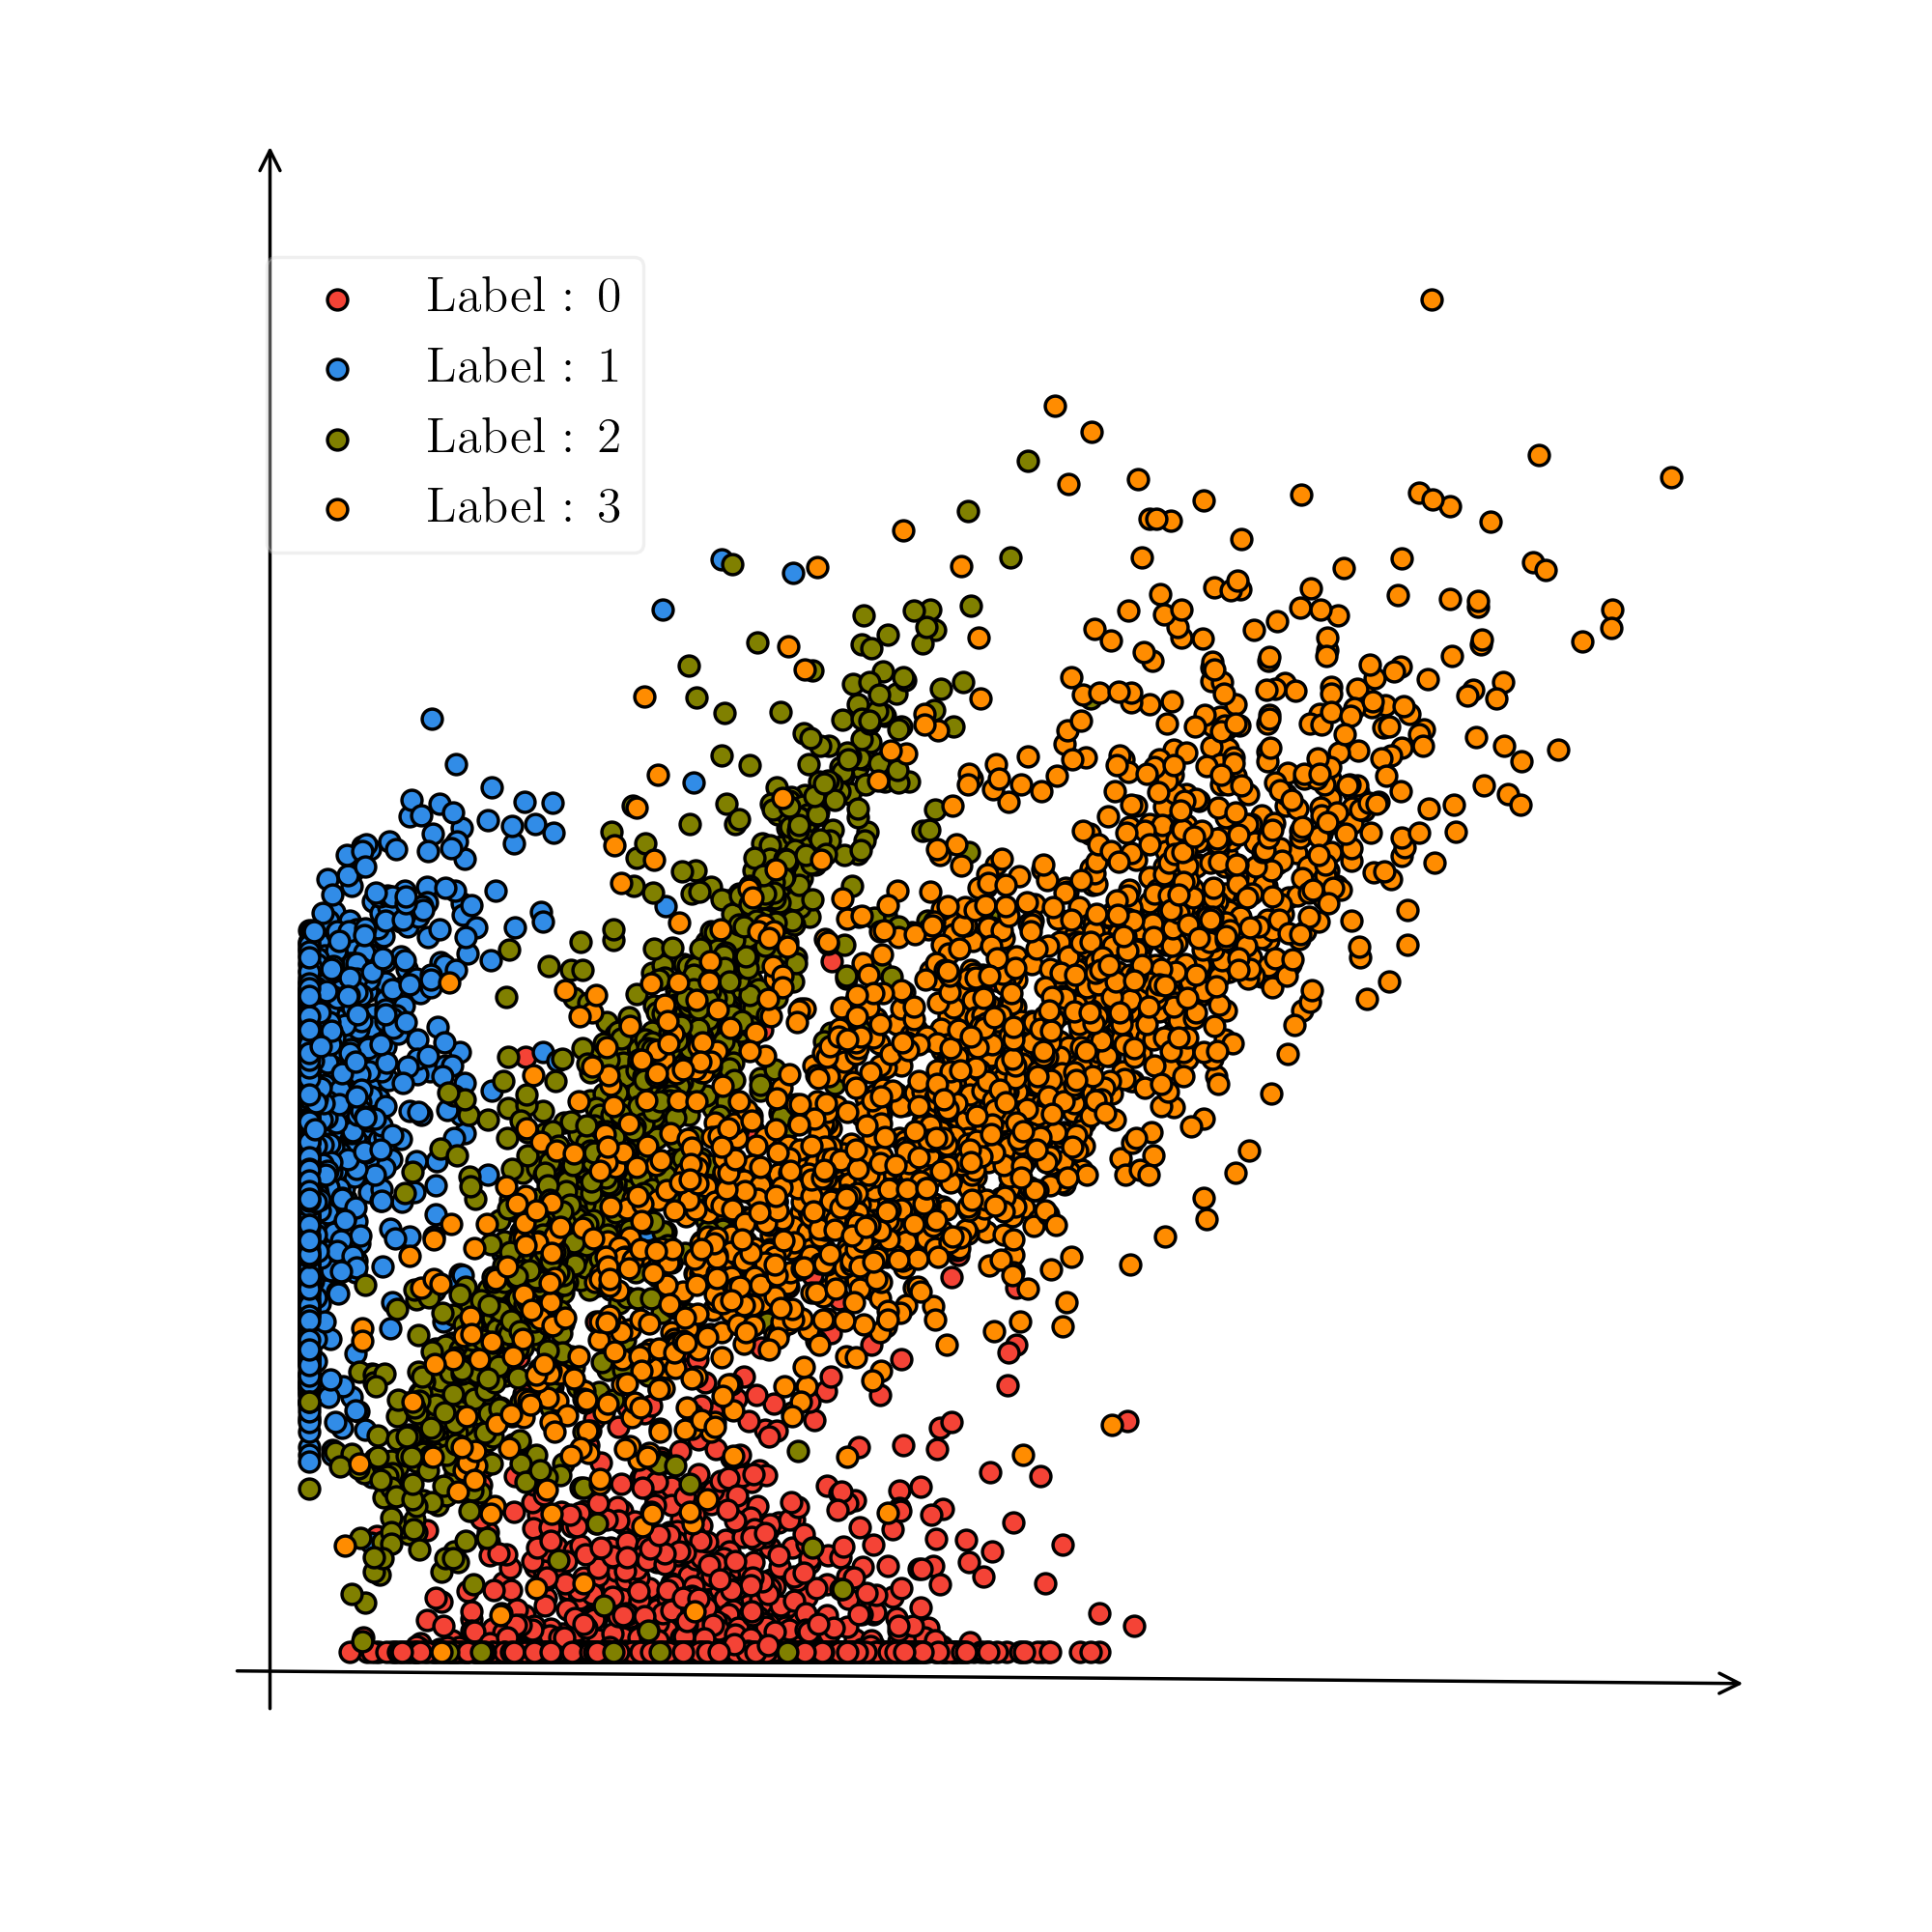
\includegraphics[width=0.7\textwidth]{figures/MNIST_l2_full.png}
			\caption{MNIST : Layer 2}
		\end{figure}
	\end{columns}
\end{frame}


\begin{frame}{}{Deep Learning and Neural Networks}
	Ok, Deep Learning is a model that learns a good representation of the feature. But how?
	\begin{itemize}
		\item How does it work ?
		\item How can we build a model ?
		\item How does it learn ?
	\end{itemize}
\end{frame}

\section{Neural Networks Fundamentals}
\begin{frame}
	Typically, a neural network is defined as a computational model composed of interconnected nodes, organised into layers, that perform transformations on input data.
	\begin{figure}
		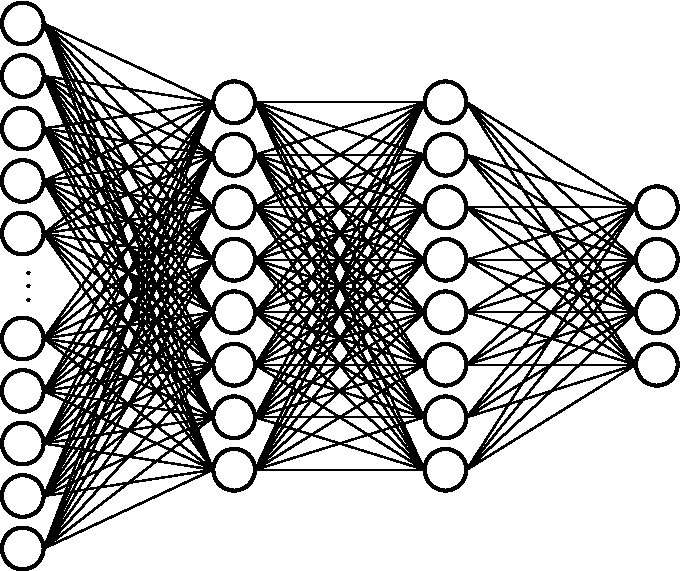
\includegraphics[width = 0.5\textwidth]{figures/ANN.pdf}
	\end{figure}
	Let's see what the interconnected nodes, the layers and the transformations are.

\end{frame}
\subsection{Neurons}
\begin{frame}{}{Neurons}
	If we consider that the Neural Network is a function $f:\mathbb{R}^d\rightarrow \mathbb{R}^m$:
	\begin{figure}
		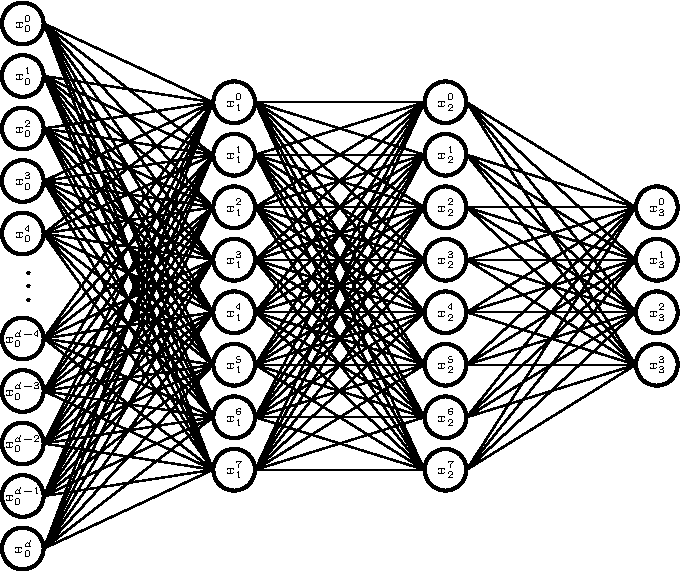
\includegraphics[width = 0.5\textwidth]{figures/ANN_neurons.pdf}
	\end{figure}
	A \alert{Neuron} is a processing unit that receives input, performs a computation, and produces an output. Here, the inputs are $x_{i-1}$ and the output is $x_{i}^k$.
\end{frame}

\begin{frame}
	For example, with an image dataset, the image can be flattened:
	\begin{figure}
		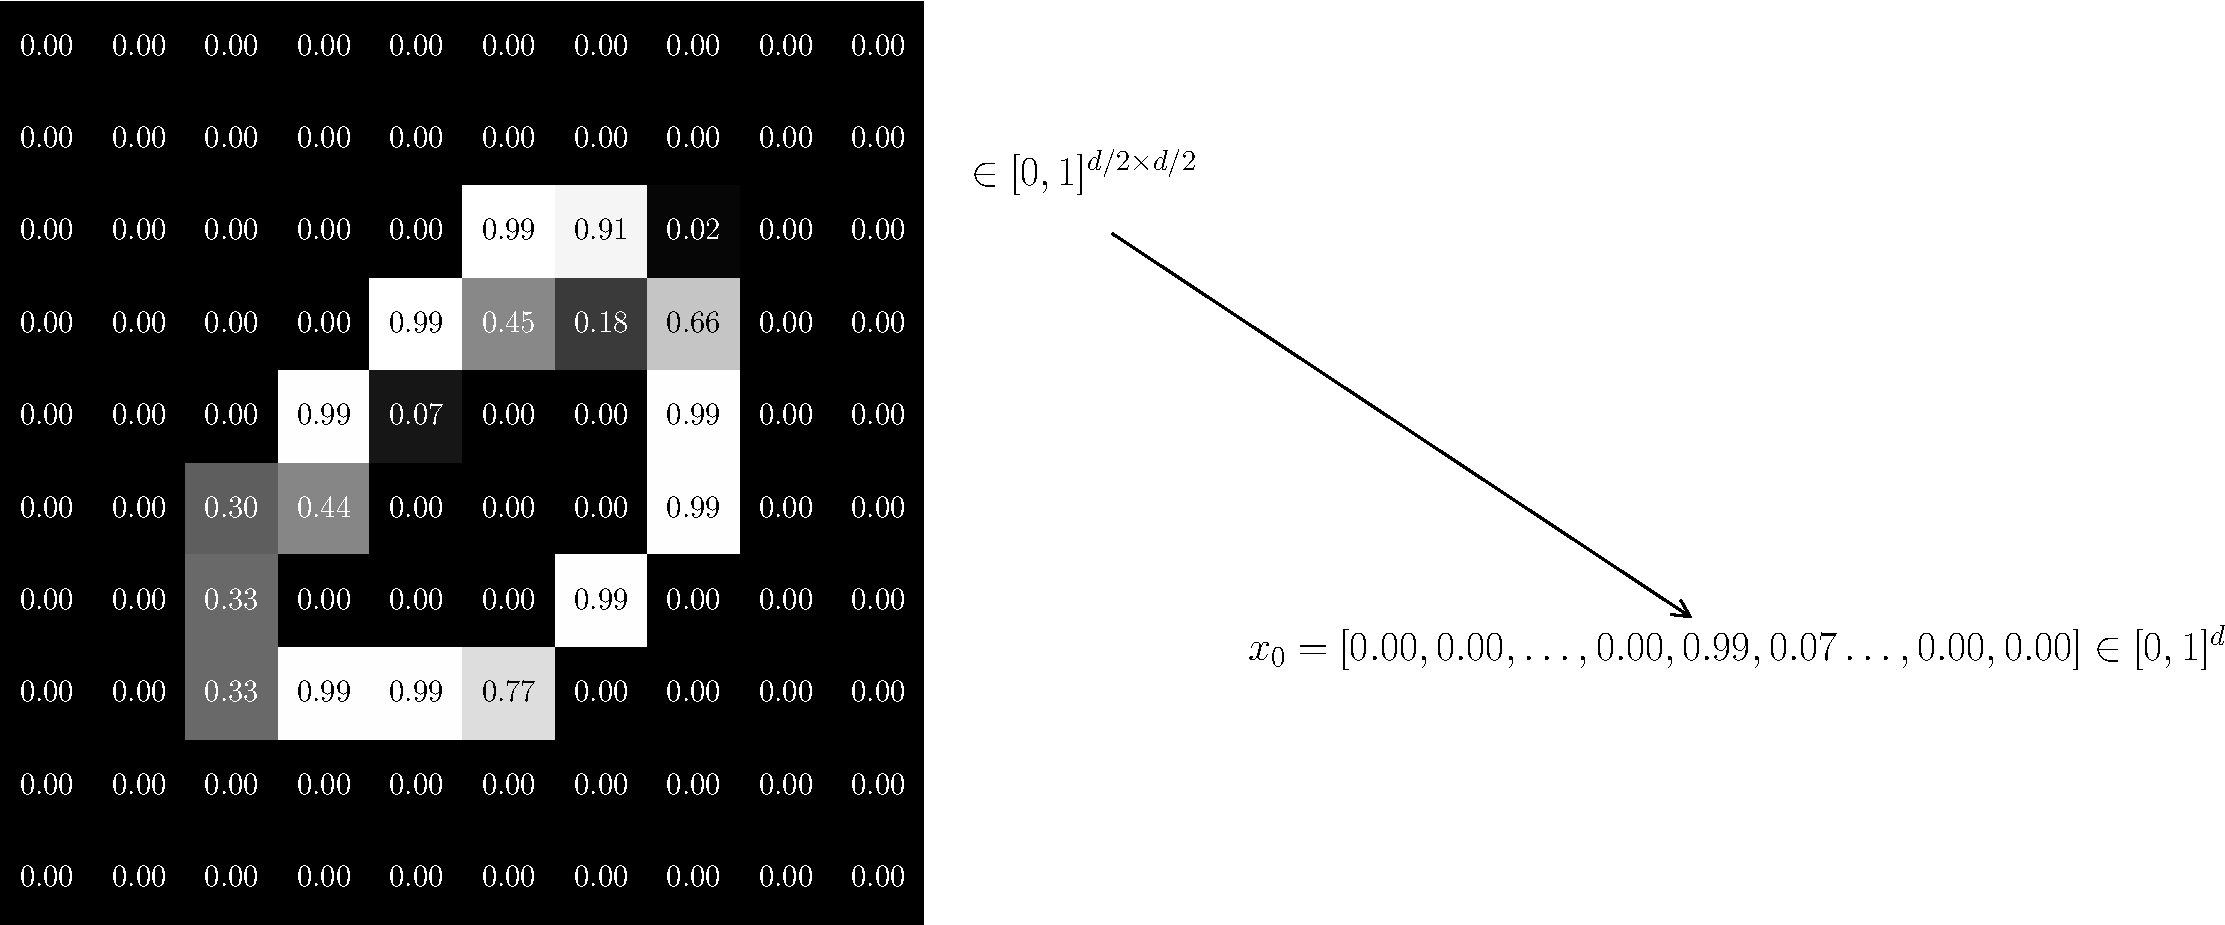
\includegraphics[width = 0.9\textwidth]{figures/mnist2ANN.pdf}
	\end{figure}
\end{frame}

\subsection{Layers}

\begin{frame}
	\begin{columns}[c,onlytextwidth]
		\column{0.3\textwidth}
		A layer $i$ is defined by a matrix $A_i\in\mathbb{R}^{k_{i-1}\times k_{i}}$, a vector $b_i\in\mathbb{R}^{k_{i}}$ and a nonlinear function $\sigma_i:\mathbb{R}\mapsto\mathbb{R}$. The transformation made by a layer is:
		$$x_i =\sigma_i\left(A_ix_{i-1}+b_i\right).$$
		The non-linear function $\sigma_i$ the \alert{activation function}.
		\column{0.7\textwidth}
		\begin{figure}
			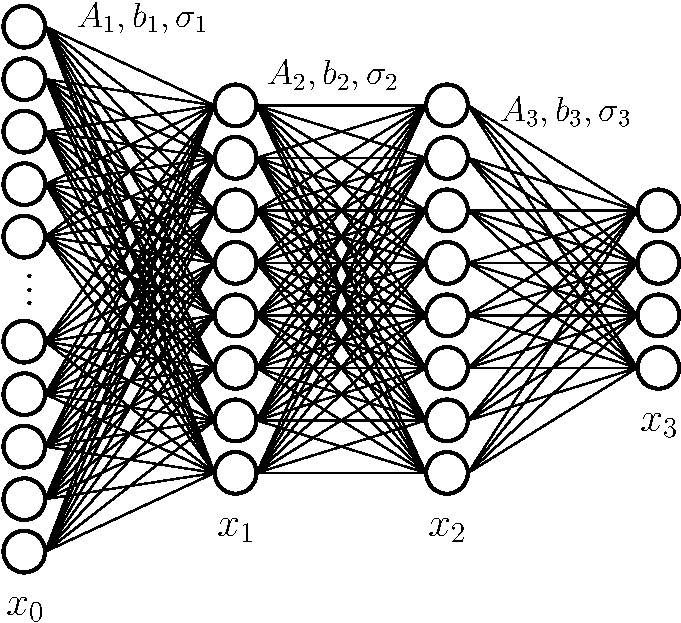
\includegraphics[width = 0.7\textwidth]{figures/ANN_layers.pdf}
		\end{figure}
	\end{columns}
\end{frame}

\begin{frame}
	\begin{columns}[c,onlytextwidth]
		\column{0.3\textwidth}
		A layer $i$ is defined as a matrix $A_i\in\mathbb{R}^{k_{i-1}\times k_{i}}$, a vector $b_i\in\mathbb{R}^{k_{i}}$ and a nonlinear function $\sigma_i:\mathbb{R}\mapsto\mathbb{R}$. The transformation made by a layer is:
		$$x_i^k =\sigma_i\left(\sum_{l=1}^{k_i} \left[A_i\right]_{l,k} x_{i-1}+\left[b_i\right]_k\right).$$
		The non-linear function $\sigma_i$ the \alert{activation function}.
		\column{0.7\textwidth}
		\begin{figure}
			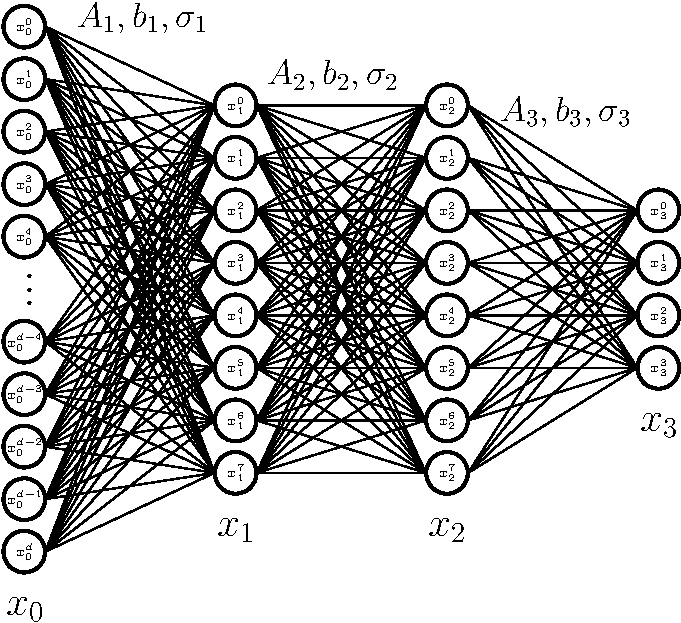
\includegraphics[width = 0.7\textwidth]{figures/ANN_complete.pdf}
		\end{figure}
	\end{columns}
\end{frame}



\subsection{Activation Functions}

\begin{frame}
	The activation functions play a crucial role in the implementation of deep neural networks, as they allow them to approximate any continuous function, as stated by the Universal Approximation Theorem.
	We can list some activation function that are commonly used :
	\begin{itemize}
		\item Linear
		\item Sigmoid
		\item Hyperbolic Tangent
		\item Rectified Linear Unit (ReLU)
		\item Leaky Rectified Linear Unit (Leaky ReLU)
		\item Exponential Linear Unit (ELU)
		\item Sigmoid-Weighted Linear Unit (Swish)
		\item Softmax
	\end{itemize}
\end{frame}

\begin{frame}{}{Linear}
	\begin{columns}[c,onlytextwidth]
		\column{0.3\textwidth}
		\begin{itemize}
			\item Linear activation Function:
			      $$
				      \sigma(x) = x
			      $$
			\item Final activation
			\item Use case : Regression
		\end{itemize}
		\column{0.7\textwidth}

		\begin{figure}
			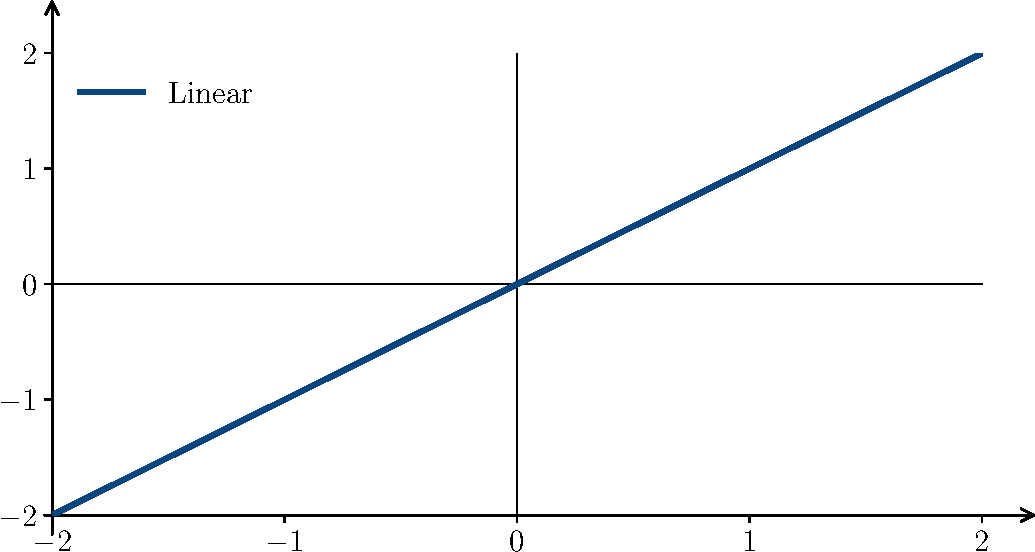
\includegraphics[width = 0.8\textwidth]{figures/linear.pdf}
		\end{figure}
	\end{columns}
\end{frame}

\begin{frame}{}{Sigmoid}
	\begin{columns}[c,onlytextwidth]
		\column{0.3\textwidth}
		\begin{itemize}
			\item Sigmoid Function:
			      $$
				      \sigma(x) = \frac{1}{1+e^{-x}}
			      $$
			\item Final activation
			\item Use case : Classification
		\end{itemize}
		\column{0.7\textwidth}
		\begin{figure}
			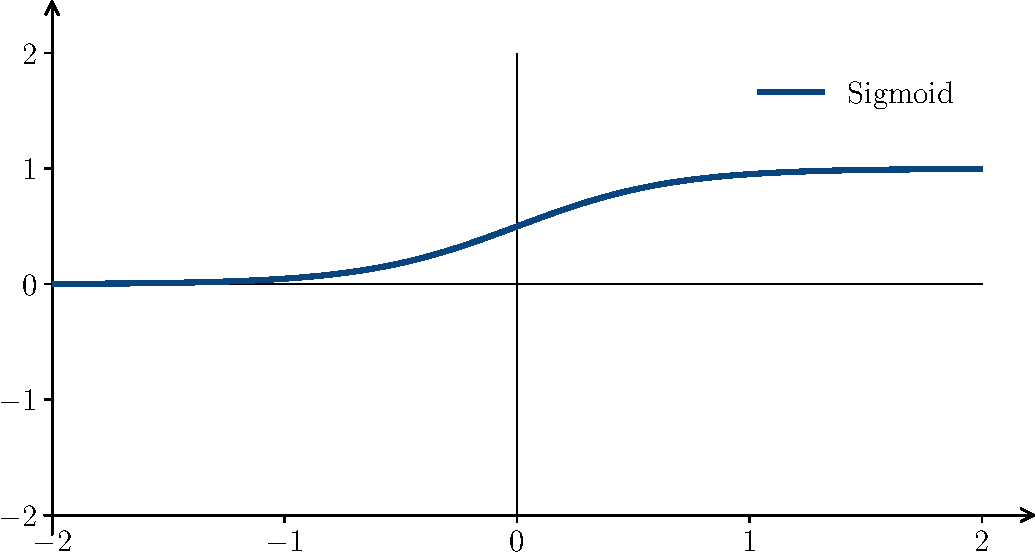
\includegraphics[width = 0.8\textwidth]{figures/sigmoid.pdf}
		\end{figure}
	\end{columns}
\end{frame}

\begin{frame}{}{Softmax}
	\begin{columns}[c,onlytextwidth]
		\column{0.3\textwidth}
		\begin{itemize}
			\item Softmax Function:
			      $$
				      \sigma(x_k) = \frac{e^{x_k}}{\sum_{i=1}^{k_i}e^{x_i}}
			      $$
			\item Final activation
			\item Use case : Multi-class Classification
		\end{itemize}
		\column{0.7\textwidth}
		\begin{figure}
			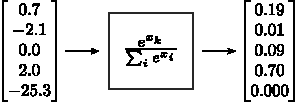
\includegraphics[width = 0.8\textwidth]{figures/softmax.pdf}
		\end{figure}
	\end{columns}
\end{frame}

\begin{frame}{}{Hyperbolic Tangent}
	\begin{columns}[c,onlytextwidth]
		\column{0.3\textwidth}
		\begin{itemize}
			\item Hyperbolic Tangent
			      $$
				      \sigma(x) = \frac{e^x-e^{-x}}{e^x+e^{-x}}
			      $$
			\item Final activation
			\item Use case : Generative task
		\end{itemize}
		\column{0.7\textwidth}
		\begin{figure}
			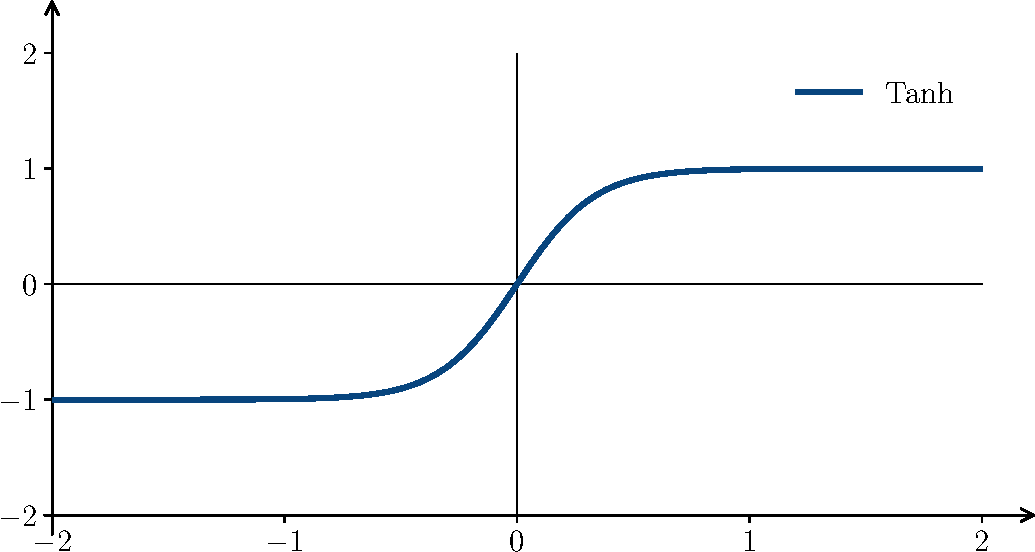
\includegraphics[width = 0.8\textwidth]{figures/tanh.pdf}
		\end{figure}
	\end{columns}
\end{frame}


\begin{frame}{}{ReLU}
	\begin{columns}[c,onlytextwidth]
		\column{0.3\textwidth}
		\begin{itemize}
			\item  Rectified Linear Unit (ReLU):
			      $$
				      \sigma(x) = \max \{0, x\}
			      $$
			\item Intermediate activation
		\end{itemize}
		\column{0.7\textwidth}
		\begin{figure}
			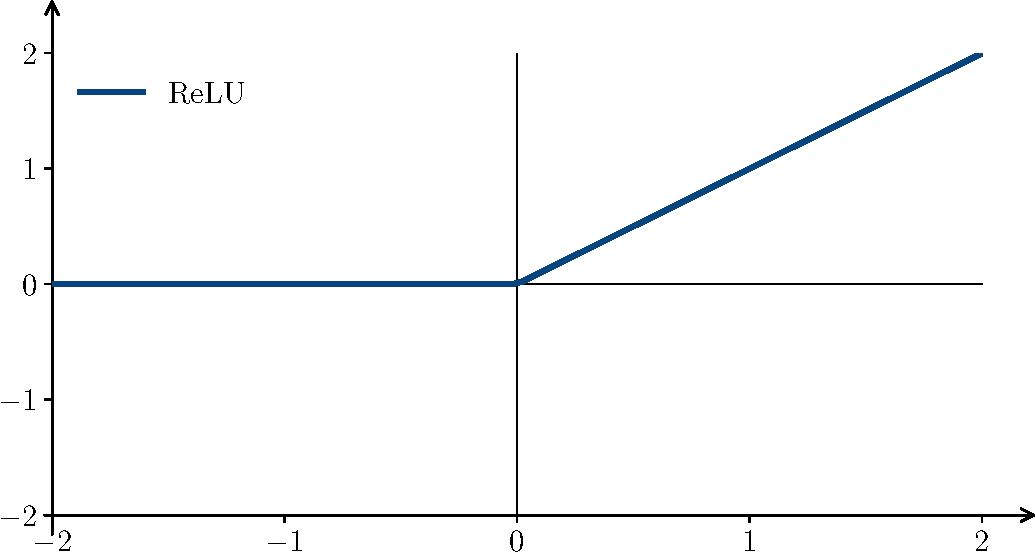
\includegraphics[width = 0.8\textwidth]{figures/relu.pdf}
		\end{figure}
	\end{columns}
\end{frame}

\begin{frame}{}{Leaky ReLU}
	\begin{columns}[c,onlytextwidth]
		\column{0.3\textwidth}
		\begin{itemize}
			\item Leaky  Rectified Linear Unit (Leaky ReLU):
			      $$
				      \sigma(x) = \max \{\alpha x, x\}
			      $$
			\item Intermediate activation
		\end{itemize}
		\column{0.7\textwidth}
		\begin{figure}
			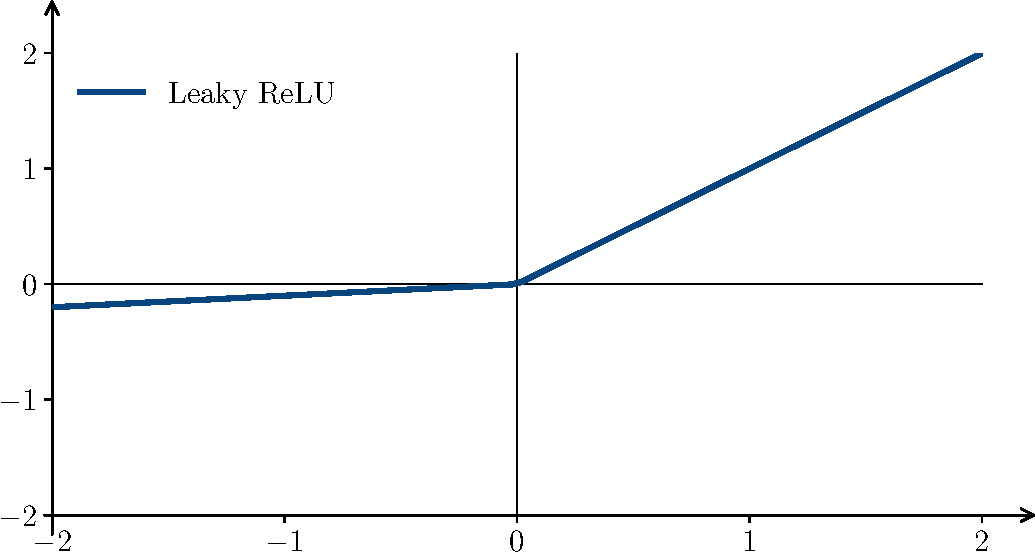
\includegraphics[width = 0.8\textwidth]{figures/leakyrelu.pdf}
		\end{figure}
	\end{columns}
\end{frame}

\begin{frame}{}{ELU}
	\begin{columns}[c,onlytextwidth]
		\column{0.3\textwidth}
		\begin{itemize}
			\item Exponential Linear Unit (ELU):
			      $$
				      \sigma(x) = \begin{cases}
					      \alpha(e^x-1) \quad \mbox{if }x<0, \\
					      x \quad \mbox{if }x\geq0.
				      \end{cases}
			      $$
			\item Intermediate activation
		\end{itemize}
		\column{0.7\textwidth}
		\begin{figure}
			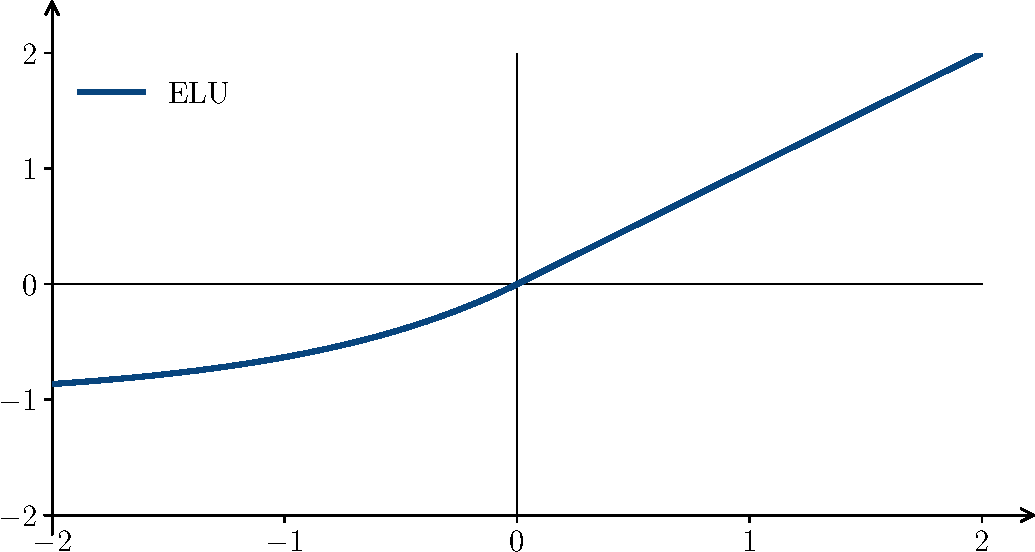
\includegraphics[width = 0.8\textwidth]{figures/elu.pdf}
		\end{figure}
	\end{columns}
\end{frame}

\begin{frame}{}{Swish}
	\begin{columns}[c,onlytextwidth]
		\column{0.3\textwidth}
		\begin{itemize}
			\item Sigmoid-Weighted Linear Unit (Swish):
			      $$
				      \sigma(x) = \frac{x}{1+e^{-x}}
			      $$
			\item Intermediate activation
		\end{itemize}
		\column{0.7\textwidth}
		\begin{figure}
			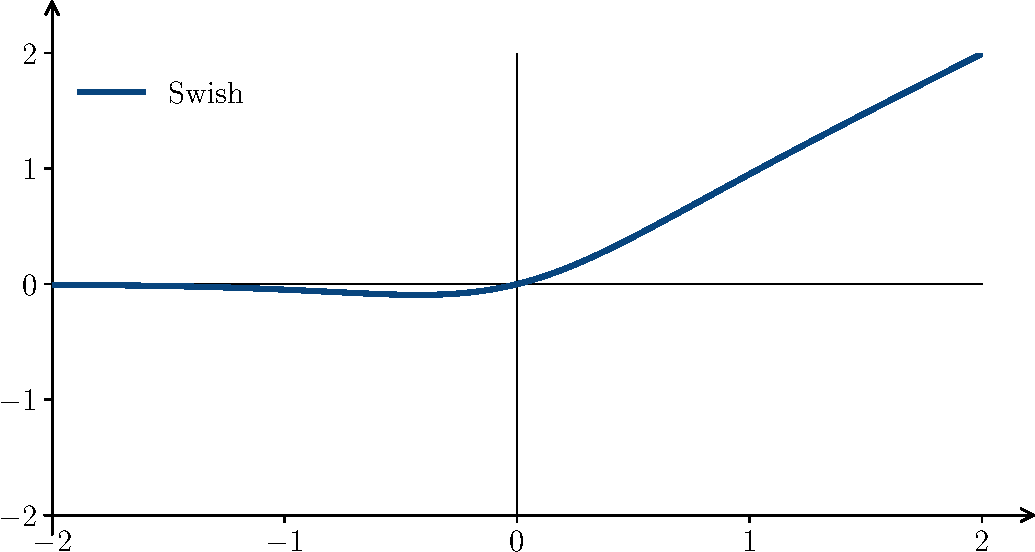
\includegraphics[width = 0.8\textwidth]{figures/swish.pdf}
		\end{figure}
	\end{columns}
\end{frame}


\section{The Multi-layer Perceptron (MLP)}

\begin{frame}
	Having discussed the structure of a neural network, we will proceed to examine the process of training a model for a specific task. As an illustration, we will consider the example of a Multilayer Perceptron.The two intermediate activation functions are ReLUs and the final activation is a softmax to perform multi-class classification on MNIST. We will consider only 4 classes.
	\begin{figure}
		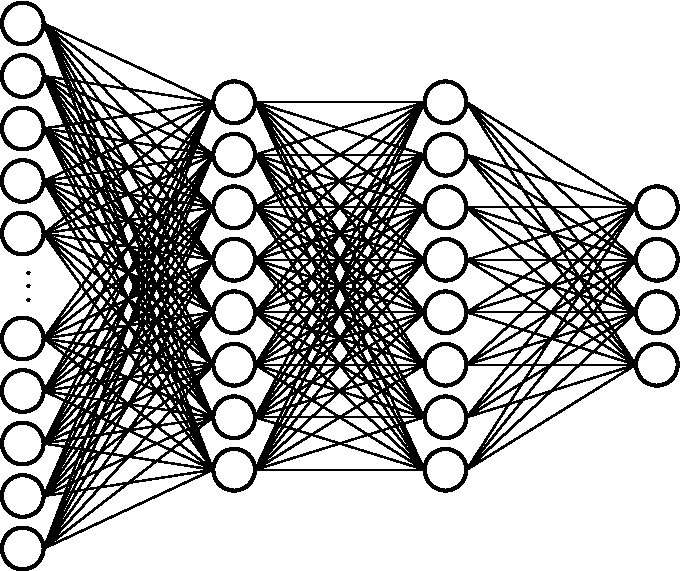
\includegraphics[width = 0.45\textwidth]{figures/ANN.pdf}
	\end{figure}
\end{frame}

\subsection{The first Deep Learning Model}
\begin{frame}
	To introduce the training process, we will consider a 3 layers MLP trained to minimise a loss $\cal L$ over a given a dataset $\cal D$. The model $f_{\theta}$ is parameterised by a vector $\theta=\left\{A_1, A_2, A_3, b_1, b_2, b_3\right\}$:
	$$
		\theta^* = \arg\min_\theta \mathcal{L}( \theta, \mathcal{D})
	$$
	\begin{figure}
		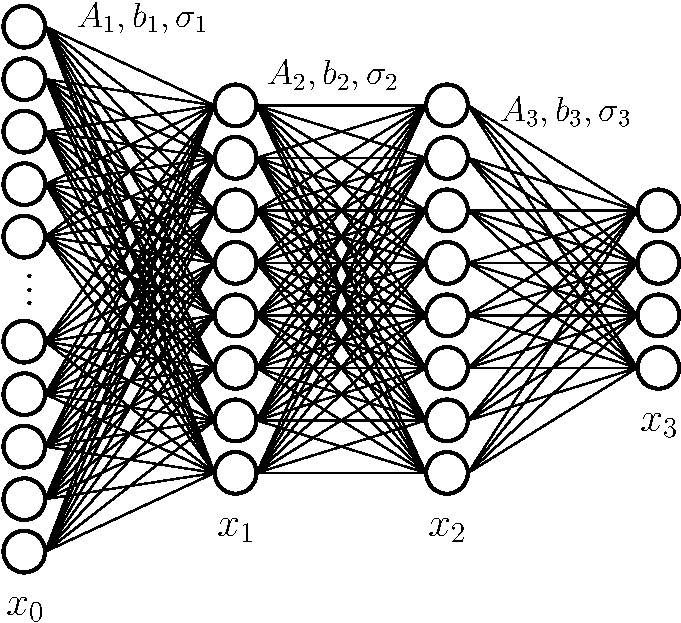
\includegraphics[width = 0.4\textwidth]{figures/ANN_layers.pdf}
	\end{figure}

\end{frame}

\subsection{Stochastic Gradient Descent}

\begin{frame}
	Stochastic gradient descent (SGD) is widely used in deep learning instead of traditional gradient descent due to its efficiency and faster convergence rate. SGD updates the model parameters after computing the gradient of the loss function with respect to each parameter using only a single randomly selected sample. This leads to a faster convergence rate and improved optimization compared to traditional gradient descent, which uses the entire training dataset to compute the gradient at each iteration.

	$$
		\theta^* = \arg \min_\theta \mathcal{L}( \theta, \mathcal{D}) =  \arg \min_\theta \mathbb{E}_{x\sim\mathcal{D}} \left[l(x, f_{\theta}(x))\right]
	$$

\end{frame}
\begin{frame}
	Theoretically the algorithm is the following: \vspace{2cm}
	\begin{algorithm}[H]
		\begin{algorithmic}[1]
			\REQUIRE Given a loss function $l$, a dataset $\mathcal{D}=\{x_1,x_2, \dots, x_N\}$ and a learning rate $\lambda$
			\STATE Initialize parameters $\theta$
			\WHILE {$\theta$ has not converged}
			\FOR{$i = 1$ to $N$}
			\STATE Randomly select $x_i$ from the dataset
			\STATE Compute gradient of the loss with respect to $\theta$: $\nabla_{\theta} l(x_i, f_{\theta}(x_i))$
			\STATE Update parameters $\theta = \theta - \lambda \nabla_{\theta} l(x_i, f(x_i))$
			\ENDFOR
			\ENDWHILE

			\RETURN $\theta$
		\end{algorithmic}
	\end{algorithm}
\end{frame}

\begin{frame}{}{SGD in mini-batch}
	In practice the algorithm is modified to use mini-batches of data instead of single samples. This is done to improve the stability of the optimization process and reduce the variance of the gradient estimates. The algorithm is as follows:

	\vspace{1cm}
	\begin{algorithm}[H]
		\begin{algorithmic}[1]
			\REQUIRE Given a loss function $l$, a dataset $\mathcal{D}=\{x_1,x_2, \dots, x_N\}$, a learning rate $\lambda$ and a batch size $b$
			\STATE Initialize parameters $\theta$
			\STATE Initialize the number of batches $B = \left\lfloor \frac{N}{b}\right\rfloor$
			\WHILE {$\theta$ has not converged}
			\FOR{$i = 1$ to $B$}
			\STATE Randomly select a mini-batch of $b$ samples from the dataset
			\STATE Compute gradient of the loss with respect to $\theta$: $\frac{1}{B}\sum_{i=1}^{B} \nabla_{\theta} l(x_i, f_{\theta}(x_i))$
			\STATE Update parameters $\theta = \theta - \lambda  \frac{1}{B}\sum_{i=1}^{B} \nabla_{\theta}l(x_i, f(x_i))$
			\ENDFOR
			\ENDWHILE
			\RETURN $\theta$
		\end{algorithmic}
	\end{algorithm}
\end{frame}


\subsection{Back-propagation}
\begin{frame}
	At every step $t$ of the gradient descent, setting a learning rate $\lambda$, the parameter $\theta$ is updated as:
	$$
		\theta_{t+1}  = \theta_t - \lambda \nabla_{\theta} l(f(x_i), y_i)
	$$
	But $\theta=\{A_1, A_2, A_3, b_1, b_2, b_3\}$ and the gradient is computed with respect to each parameter.
	\begin{figure}
		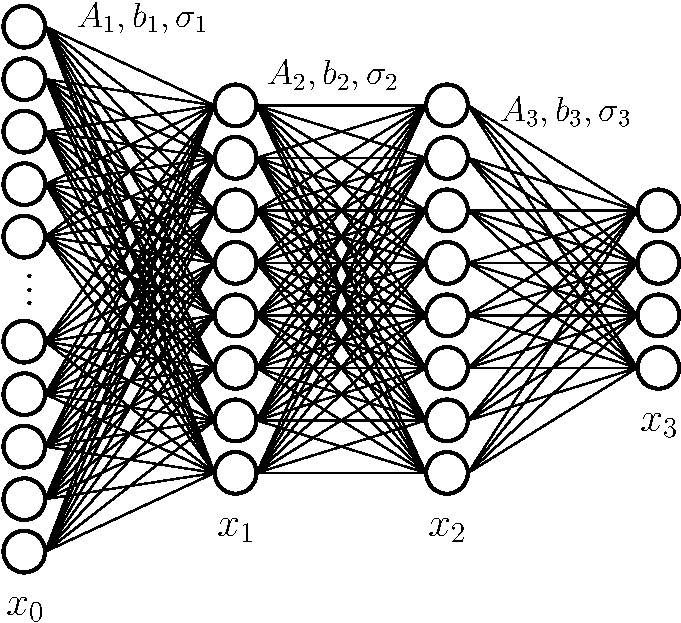
\includegraphics[width = 0.4\textwidth]{figures/ANN_layers.pdf}
	\end{figure}
\end{frame}

\begin{frame}
	First we will consider a single data point $x$, the loss will depend on the output only: $ l(f(x))$.\newline


	$f$ is a layered composed function. Let us focus on the last layer:
	\begin{align*}
		f(x) & = x_3 = \sigma_3(A_3 x_2+b_3)
	\end{align*}
	Therefore:
	\begin{align*}
		l(f(x)) = l\left(\sigma_3\left(A_3x_2+b_3\right)\right)
	\end{align*}
	To minimise the loss, we have to act on $A_3$, $b_3$ and $x_2$.
\end{frame}

\begin{frame}{}{Back-propagation}
	Let us look at the gradients with respect to $A_3$:
	\begin{align*}
		\frac{\partial l}{\partial A_3} & = \frac{\partial l}{\partial x_3}\frac{\partial x_3}{\partial A_3} =l'(x_3)\frac{\partial \sigma_3\left(A_3x_2+b_3\right)}{\partial A_3} = l'(x_3)\sigma_3'\left(A_3x_2+b_3\right)\frac{\partial \left[A_3x_2+b_3\right]}{\partial A_3} \\
		                                & = \underbrace{l'(x_3)}_{\in\mathbb{R}}\:\underbrace{\sigma_3'\left(A_3x_2+b_3\right)}_{\in\mathbb{R}^{k_i\times 1}}\underbrace{x_2^T}_{\in\mathbb{R}^{1\times k_{i-1}}}
	\end{align*}
	and therefore:
	\begin{align*}
		A_3 \leftarrow A_3 - \lambda l'(x_3)\sigma_3'\left(A_3x_2+b_3\right)x_2^T.
	\end{align*}
	We need to keep in memory the latent values of $x$, i.e. $x_2$.
\end{frame}

\begin{frame}{}{Back-propagation}
	Let us look at the gradients with respect to $A_2$:
	\begin{align*}
		\frac{\partial l}{\partial A_2} & = \frac{\partial l}{\partial x_2}\frac{\partial x_2}{\partial A_2}                                                    \\
		                                & =\frac{\partial l}{\partial x_2}\frac{\partial \sigma_2\left(A_2x_1+b_2\right)}{\partial A_2}                         \\
		                                & =\frac{\partial l}{\partial x_2}\sigma_2'\left(A_2x_1+b_2\right)\frac{\partial \left[A_2x_1+b_2\right]}{\partial A_2} \\
		                                & =\frac{\partial l}{\partial x_2} \: \sigma_2'\left(A_2x_1+b_2\right)x_1^T
	\end{align*}
	which depends on $\frac{\partial l}{\partial x_2}$, we need to compute it.
\end{frame}
\begin{frame}{}{Back-propagation}
	We have to compute the gradient with respect to $x_2$:
	\begin{align*}
		\frac{\partial l}{\partial x_2} & = \frac{\partial l}{\partial x_3}\frac{\partial x_3}{\partial x_2} =l'(x_3)\frac{\partial \sigma_3\left(A_3x_2+b_3\right)}{\partial x_2} = l'(x_3)\frac{\partial \left[A_3x_2+b_3\right]}{\partial x_2}\sigma_3'\left(A_3x_2+b_3\right) \\
		                                & =l'(x_3)\:A_3^T\sigma_3'\left(A_3x_2+b_3\right)
	\end{align*}
	Therefore:
	\begin{align*}
		A_2 \leftarrow A_2 - \lambda \left[l'(x_3)A_3^T\sigma_3'\left(A_3x_2+b_3\right) \times  \sigma_2'\left(A_2x_1+b_2\right)x_1^T \right]
	\end{align*}
	The update of $A_2$ depends on $l'(x_3)$,
\end{frame}


\begin{frame}{Back-propagation}
	We have to compute the gradient with respect to $A_1$:
	\begin{align*}
		\frac{\partial l}{\partial A_1} & = \frac{\partial l}{\partial x_1}\frac{\partial x_1}{\partial A_1}                            \\
		                                & =\frac{\partial l}{\partial x_1}\frac{\partial \sigma_1\left(A_1x_0+b_1\right)}{\partial A_1} \\
		                                & =\frac{\partial l}{\partial x_1} \sigma_1'\left(A_1x_0+b_0\right)x_0^T,
	\end{align*}
	which depends on $\frac{\partial l}{\partial x_1}$, we need to compute it.
\end{frame}

\begin{frame}{Back-Propagation}
	Let us compute the gradient with respect to $x_1$:
	\begin{align*}
		\frac{\partial l}{\partial x_1} & = \frac{\partial l}{\partial x_2}\frac{\partial x_2}{\partial x_1} = \frac{\partial l}{\partial x_2}\frac{\partial \sigma_2\left(A_2x_1+b_2\right)}{\partial x_1} =  \frac{\partial l}{\partial x_2}\frac{\partial \left[A_2x_1+b_2\right]}{\partial x_1}\sigma_2'\left(A_2x_1+b_2\right) \\
		                                & = \frac{\partial l}{\partial x_2}A_2^T\sigma_2'\left(A_2x_1+b_2\right)
	\end{align*}
	Therefore:
	\begin{align*}
		A_1 \leftarrow A_1 - \lambda \left[l'(x_3)\:A_3^T\sigma_3'\left(A_3x_2+b_3\right)A_2^T\sigma_2'\left(A_2x_1+b_2\right) \times  \sigma_1'\left(A_1x_0+b_1\right)x_0^T \right]
	\end{align*}
\end{frame}

\begin{frame}{Back-Propagation}
	In other words, the update on the weights is:
	\begin{align*}
		A_3 & \leftarrow A_3 - \lambda l'(x_3)\sigma_3'\left(A_3x_2+b_3\right)x_2^T                                                                                                    \\
		A_2 & \leftarrow A_2 - \lambda \left[l'(x_3)A_3^T\sigma_3'\left(A_3x_2+b_3\right) \times  \sigma_2'\left(A_2x_1+b_2\right)x_1^T \right]                                        \\
		A_1 & \leftarrow A_1 - \lambda \left[l'(x_3)\:A_3^T\sigma_3'\left(A_3x_2+b_3\right)A_2^T\sigma_2'\left(A_2x_1+b_2\right) \times  \sigma_1'\left(A_1x_0+b_1\right)x_0^T \right]
	\end{align*}
\end{frame}



\begin{frame}
	If we look at the update of the different biases, we can easily compute the different gradient and see the updates.
	First, let us compute the gradient with respect to $b_3$:
	\begin{align*}
		\frac{\partial l}{\partial b_3} & = \frac{\partial l}{\partial x_3}\frac{\partial x_3}{\partial b_3}                                                  \\
		                                & =l'(x_3)\frac{\partial \sigma_3\left(A_3x_2+b_3\right)}{\partial b_3}                                               \\
		                                & = l'(x_3)\sigma_3'\left(A_3x_2+b_3\right)\frac{\partial \left[A_3x_2+b_3\right]}{\partial b_3}                      \\
		                                & = \underbrace{l'(x_3)}_{\in\mathbb{R}}\:\underbrace{\sigma_3'\left(A_3x_2+b_3\right)}_{\in\mathbb{R}^{k_i\times 1}}
	\end{align*}
	And thus :
	$$
		b_3 \leftarrow b_3 - \lambda l'(x_3)\sigma'\left(A_3x_2+b_3\right)
	$$
\end{frame}
\begin{frame}
	Let's move on the second layer:
	\begin{align*}
		\frac{\partial l}{\partial b_2} & = \frac{\partial l}{\partial x_2}\frac{\partial x_2}{\partial b_2}                            \\
		                                & =\frac{\partial l}{\partial x_2}\frac{\partial \sigma_2\left(A_2x_1+b_2\right)}{\partial b_2} \\
		                                & =\frac{\partial l}{\partial x_2} \sigma_2'\left(A_2x_1+b_2\right)                             \\
	\end{align*}
	And thus :
	$$
		b_2 \leftarrow b_2 - \lambda	\frac{\partial l}{\partial x_2} \sigma'\left(A_2x_1+b_2\right)
	$$
	We need to back-propagate the term $\frac{\partial l}{\partial x_2}$ computed for the first layer.
\end{frame}

\begin{frame}
	For the first layer:
	\begin{align*}
		\frac{\partial l}{\partial b_1} & = \frac{\partial l}{\partial x_1}\frac{\partial x_1}{\partial b_1}                            \\
		                                & =\frac{\partial l}{\partial x_1}\frac{\partial \sigma_1\left(A_1x_0+b_1\right)}{\partial b_1} \\
		                                & =\frac{\partial l}{\partial x_1} \sigma_1'\left(A_1x_0+b_0\right)                             \\
	\end{align*}
	And thus :
	$$
		b_1 \leftarrow b_1 - \lambda	\frac{\partial l}{\partial x_1} \sigma'\left(A_1x_0+b_1\right)
	$$
	We need to back-propagate the term $\frac{\partial l}{\partial x_1}$ computed for the second layer which has been computed with $\frac{\partial l}{\partial x_2}$ back-propagated from the first layer.
\end{frame}

\begin{frame}{}{Back-Propagation}
	To update the weights, we need to compute the gradient of the loss with respect to the output of the network, and then \textbf{back-propagate} the gradient of the loss with respect to each activation, the $\frac{\partial l}{\partial x_i}$, through the network to compute the gradients with respect to the weights and biases of each layer.
\end{frame}

\begin{frame}{}{Last Layer}
	\begin{columns}[c,onlytextwidth]
		\column{0.3\textwidth}
		We can plot the current state of the network for a given input.\newline

		The red lines show positive values for $A_i$, the blue lines represent negative values for $A_i$.
		The level of transparency is proportional to the previous neurons.
		\column{0.7\textwidth}

		\begin{figure}
			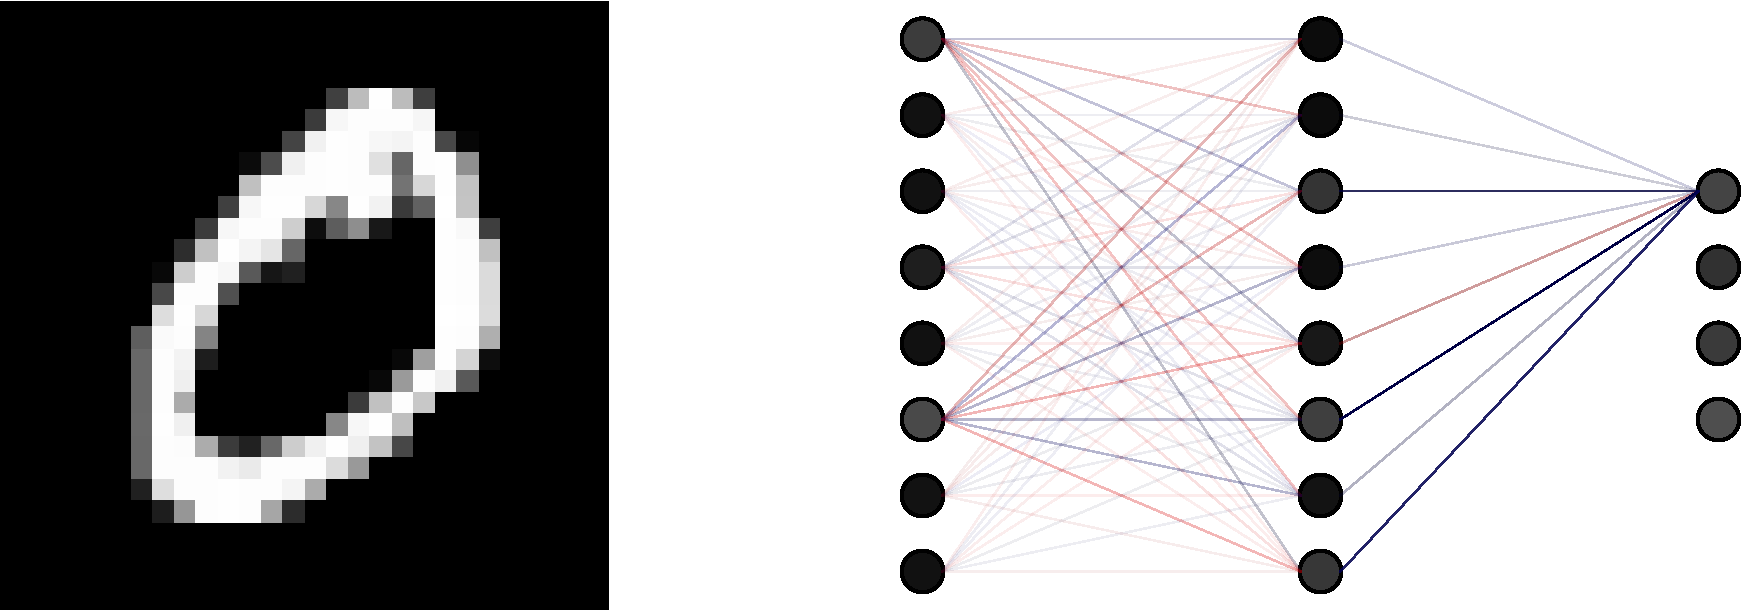
\includegraphics[width=0.9\textwidth]{figures/backpropimg0.pdf}
		\end{figure}
	\end{columns}
	\vfill
	$$
		x_3^1 = \sigma_3\left(A_{3}^{1,1}x_2^1+A_{3}^{1,2}x_2^2 +\dots+A_{3}^{1,8}x_2^8\right)
	$$
\end{frame}

\begin{frame}
	\begin{columns}[c,onlytextwidth]
		\column{0.3\textwidth}
		Iteratively, the neural networks improves its performance.
		\column{0.7\textwidth}

		\begin{figure}
			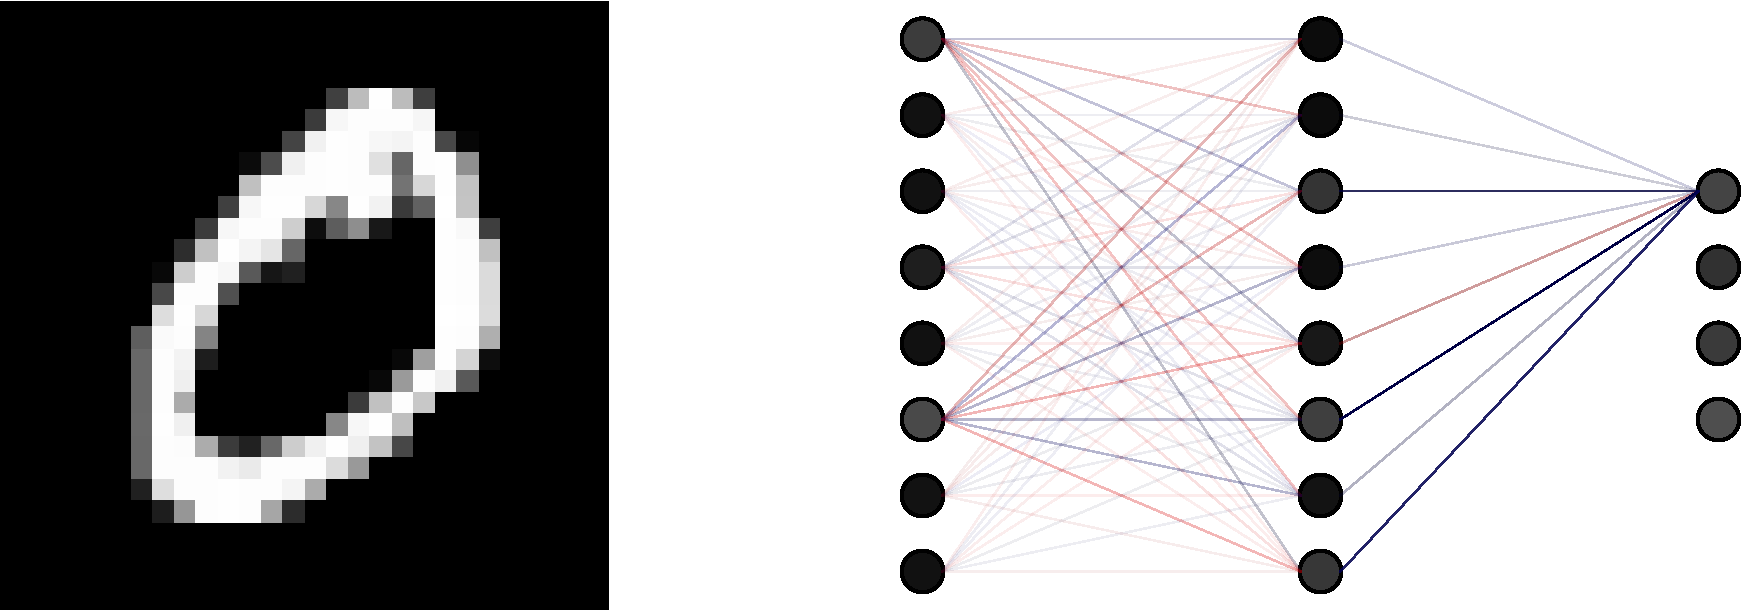
\includegraphics[width=0.9\textwidth]{figures/backpropimg0.pdf}
		\end{figure}
	\end{columns}
	\vfill
	$$
		x_3^1 = \sigma_3\left(A_{3}^{1,1}x_2^1+A_{3}^{1,2}x_2^2 +\dots+A_{3}^{1,8}x_2^8\right)
	$$
\end{frame}

\begin{frame}
	\begin{columns}[c,onlytextwidth]
		\column{0.3\textwidth}
		Iteratively, the neural networks improves its performance.
		\column{0.7\textwidth}

		\begin{figure}
			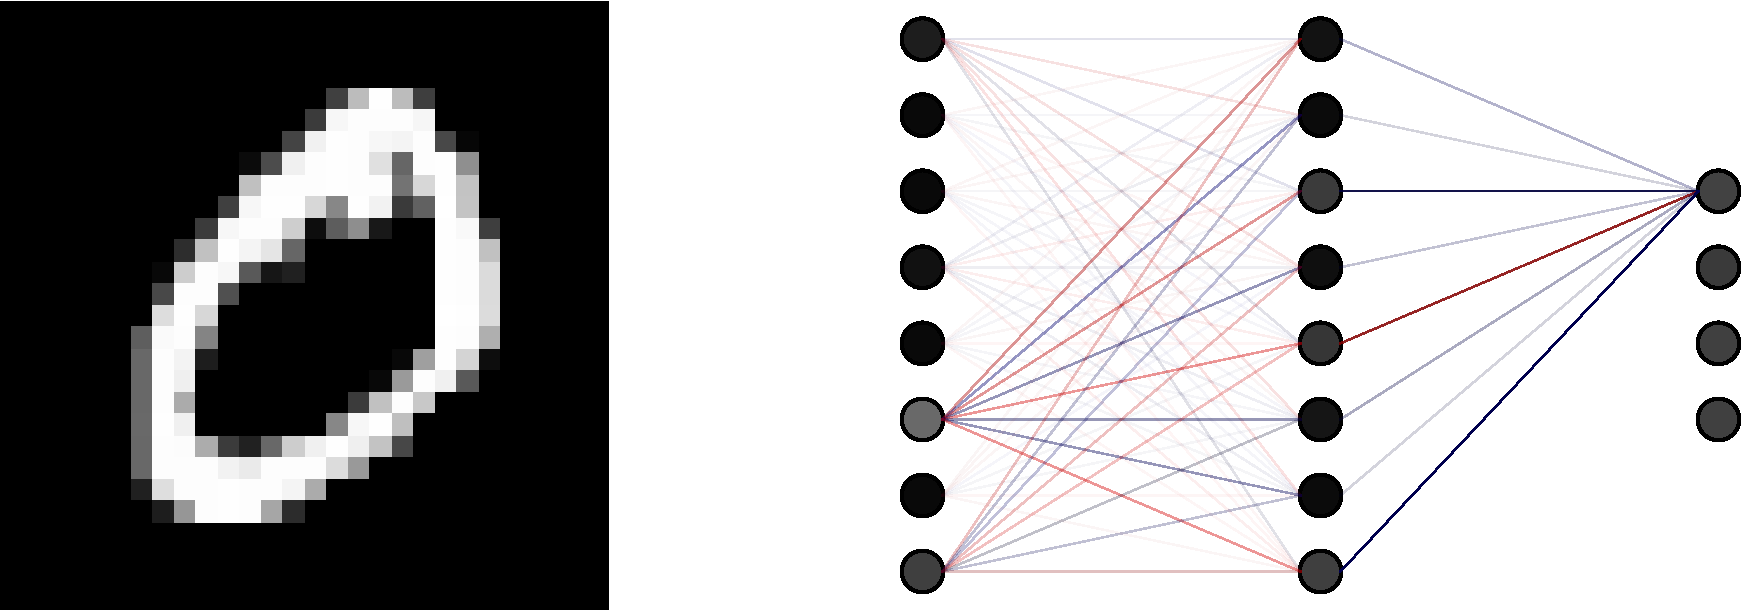
\includegraphics[width=0.9\textwidth]{figures/backpropimg1.pdf}
		\end{figure}
	\end{columns}
	\vfill
	$$
		x_3^1 = \sigma_3\left(A_{3}^{1,1}x_2^1+A_{3}^{1,2}x_2^2 +\dots+A_{3}^{1,8}x_2^8\right)
	$$
\end{frame}
\begin{frame}
	\begin{columns}[c,onlytextwidth]
		\column{0.3\textwidth}
		Iteratively, the neural networks improves its performance.
		\column{0.7\textwidth}

		\begin{figure}
			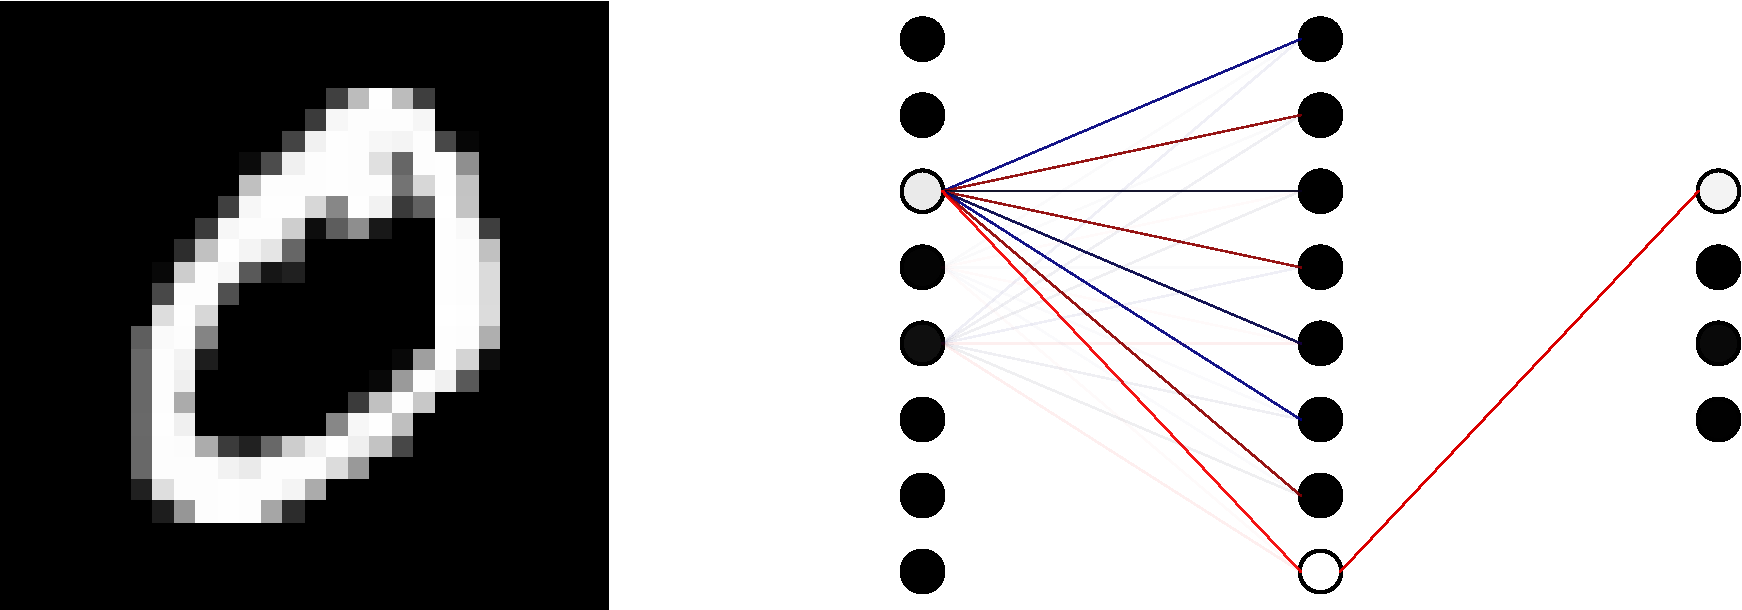
\includegraphics[width=0.9\textwidth]{figures/backpropimg2.pdf}
		\end{figure}
	\end{columns}
	\vfill
	$$
		x_3^1 = \sigma_3\left(A_{3}^{1,1}x_2^1+A_{3}^{1,2}x_2^2 +\dots+A_{3}^{1,8}x_2^8\right)
	$$
\end{frame}
\begin{frame}
	\begin{columns}[c,onlytextwidth]
		\column{0.3\textwidth}
		Iteratively, the neural networks improves its performance.
		\column{0.7\textwidth}

		\begin{figure}
			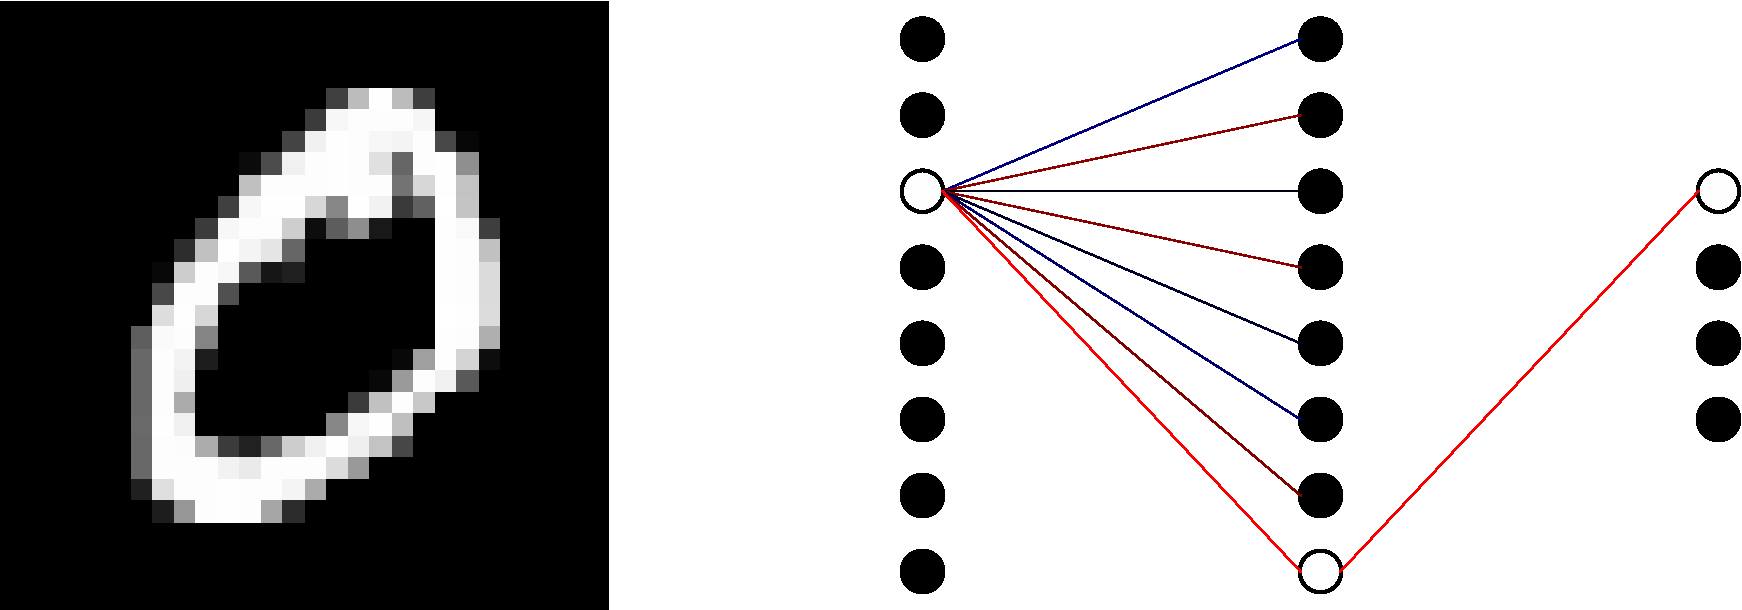
\includegraphics[width=0.9\textwidth]{figures/backpropimg3.pdf}
		\end{figure}
	\end{columns}
	\vfill
	$$
		x_3^1 = \sigma_3\left(A_{3}^{1,1}x_2^1+A_{3}^{1,2}x_2^2 +\dots+A_{3}^{1,8}x_2^8\right)
	$$
\end{frame}
\begin{frame}{}{Last Layer}
	\begin{columns}[c,onlytextwidth]
		\column{0.3\textwidth}
		We can plot the current state of the network for a given input.\newline

		Red lines show  positive values of $A_i$, Blue lines represent negative values of $A_i$.
		The level of transparency is proportional to the previous neurons.
		\column{0.7\textwidth}

		\begin{figure}
			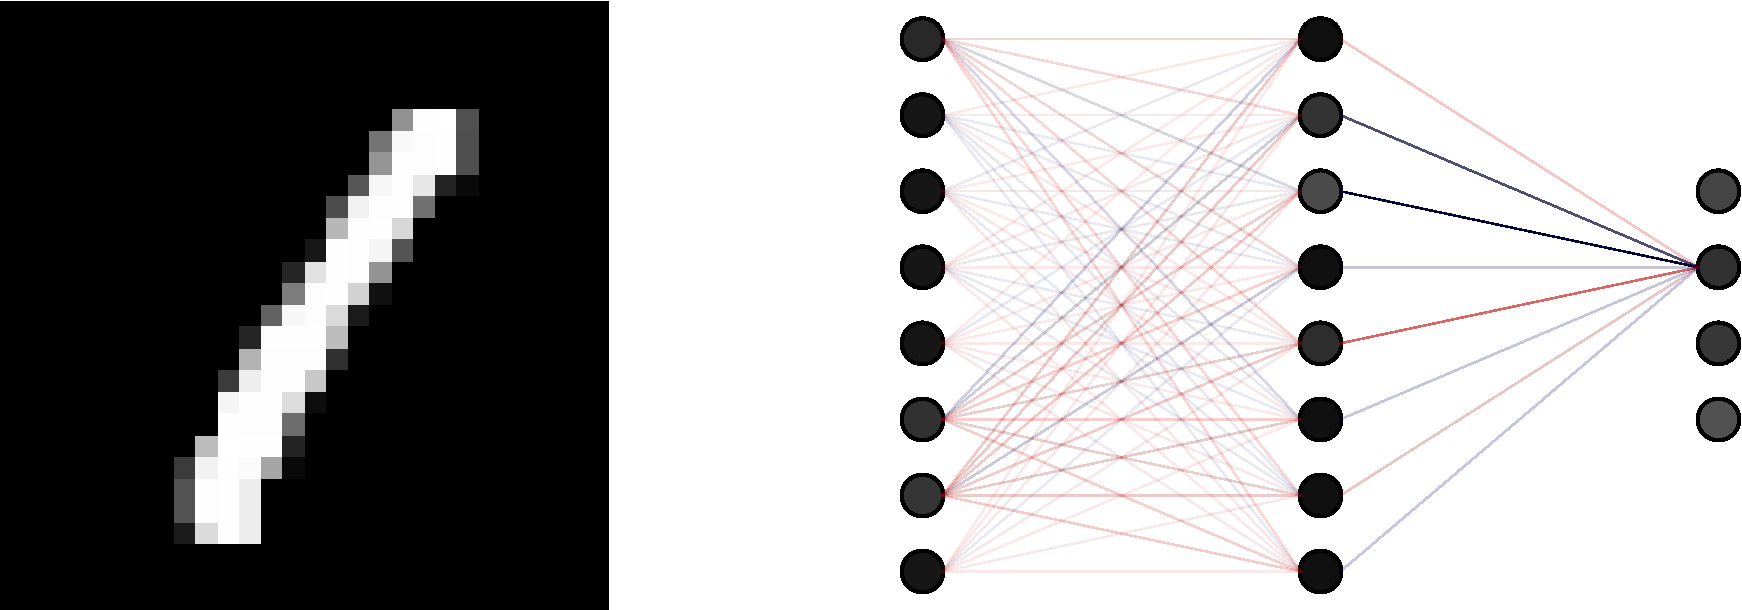
\includegraphics[width=0.9\textwidth]{figures/backpropimg01.pdf}
		\end{figure}
	\end{columns}
	\vfill
	$$
		x_3^2 = \sigma_3\left(A_{3}^{2,1}x_2^1+A_{3}^{2,2}x_2^2 +\dots+A_{3}^{2,8}x_2^8\right)
	$$
\end{frame}
\begin{frame}
	\begin{columns}[c,onlytextwidth]
		\column{0.3\textwidth}
		Iteratively, the neural networks improves its performance.
		\column{0.7\textwidth}

		\begin{figure}
			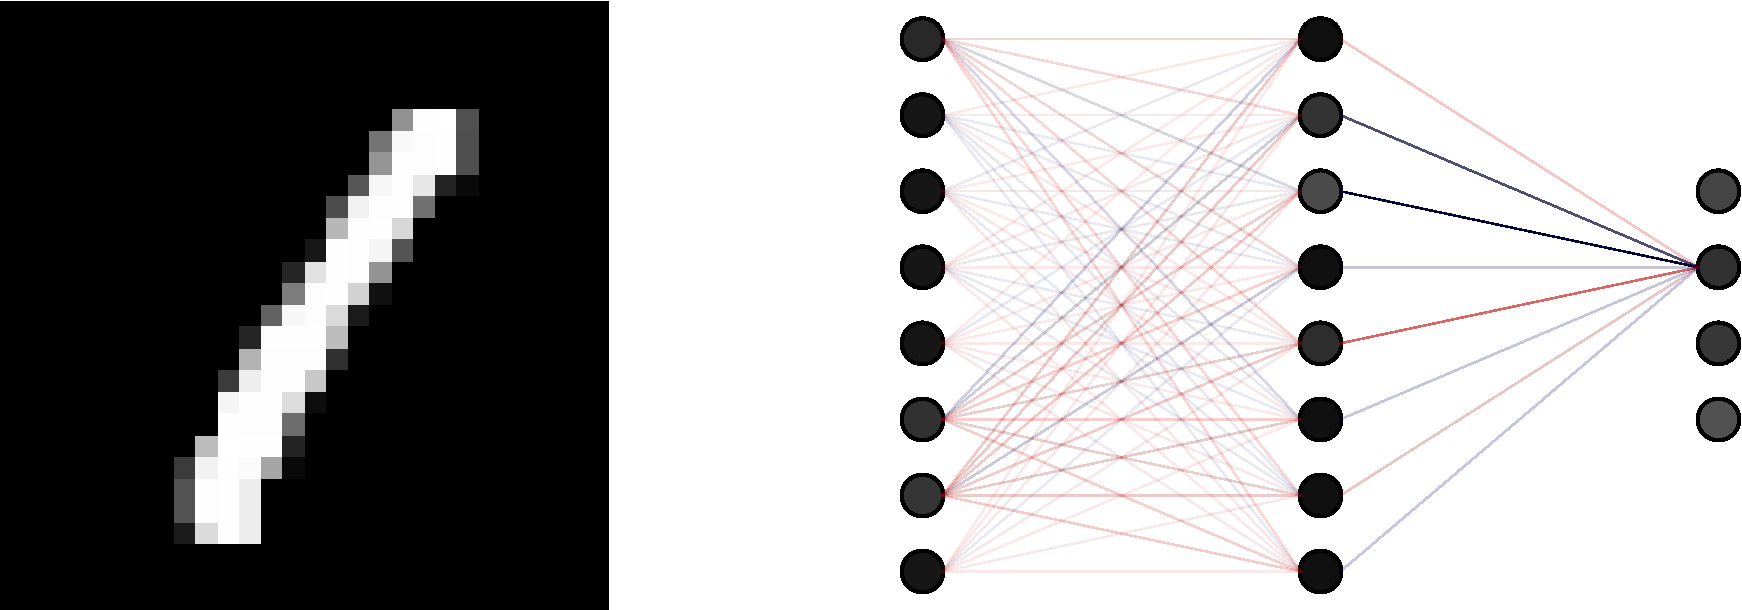
\includegraphics[width=0.9\textwidth]{figures/backpropimg01.pdf}
		\end{figure}
	\end{columns}
	\vfill
	$$
		x_3^2 = \sigma_3\left(A_{3}^{2,1}x_2^1+A_{3}^{2,2}x_2^2 +\dots+A_{3}^{2,8}x_2^8\right)
	$$
\end{frame}

\begin{frame}
	\begin{columns}[c,onlytextwidth]
		\column{0.3\textwidth}
		Iteratively, the neural networks improves its performance.
		\column{0.7\textwidth}

		\begin{figure}
			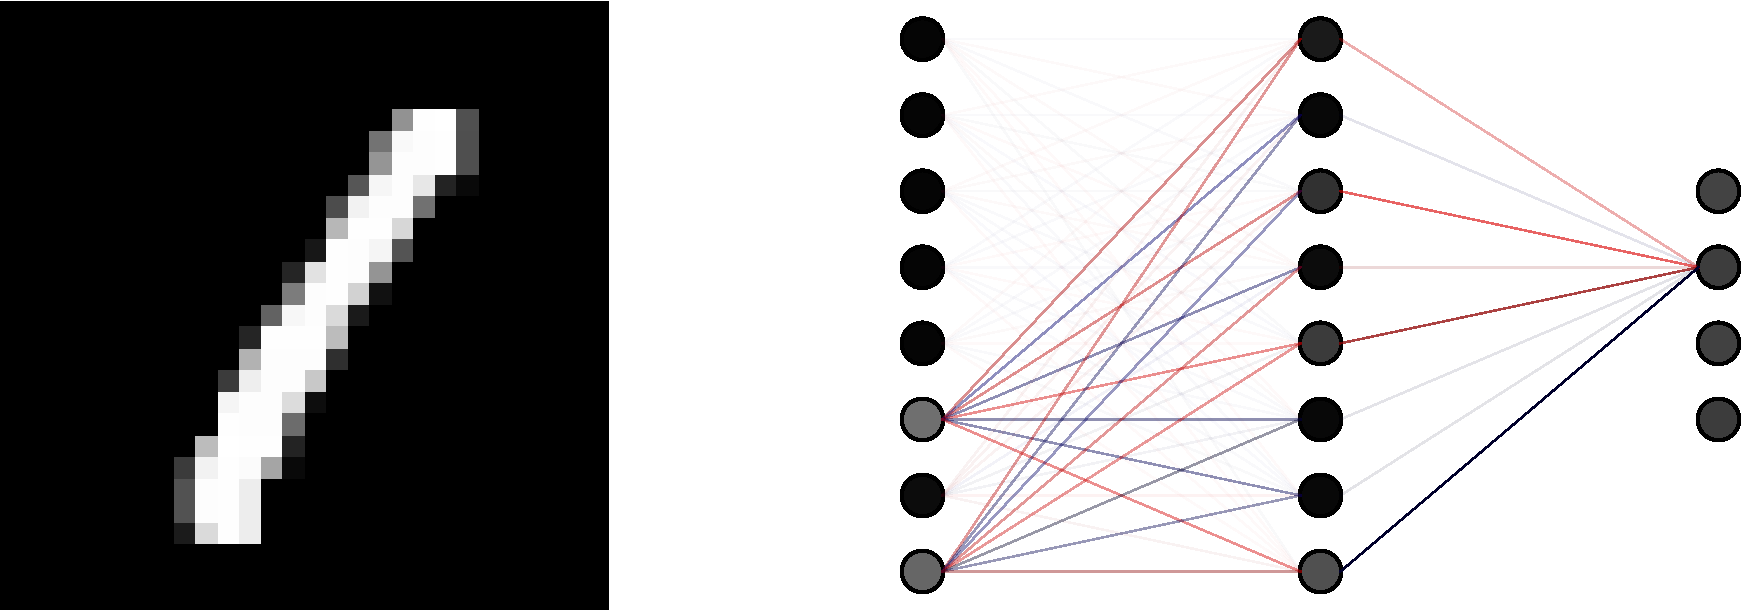
\includegraphics[width=0.9\textwidth]{figures/backpropimg11.pdf}
		\end{figure}
	\end{columns}
	\vfill
	$$
		x_3^2 = \sigma_3\left(A_{3}^{2,1}x_2^1+A_{3}^{2,2}x_2^2 +\dots+A_{3}^{2,8}x_2^8\right)
	$$
\end{frame}
\begin{frame}
	\begin{columns}[c,onlytextwidth]
		\column{0.3\textwidth}
		Iteratively, the neural networks improves its performance.
		\column{0.7\textwidth}

		\begin{figure}
			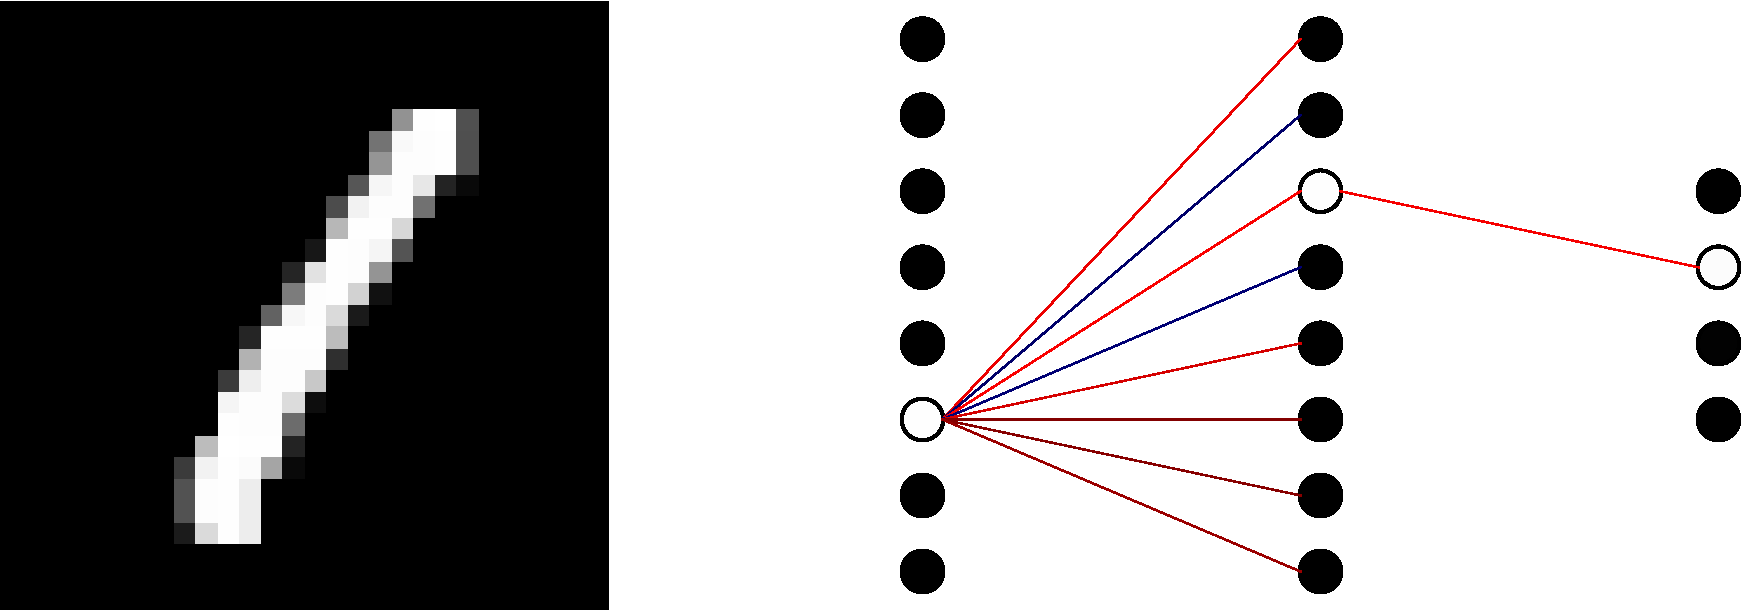
\includegraphics[width=0.9\textwidth]{figures/backpropimg13.pdf}
		\end{figure}
	\end{columns}
	\vfill
	$$
		x_3^2 = \sigma_3\left(A_{3}^{2,1}x_2^1+A_{3}^{2,2}x_2^2 +\dots+A_{3}^{2,8}x_2^8\right)
	$$
\end{frame}
\begin{frame}
	\begin{columns}[c,onlytextwidth]
		\column{0.3\textwidth}
		Iteratively, the neural networks improves its performance.
		\column{0.7\textwidth}

		\begin{figure}
			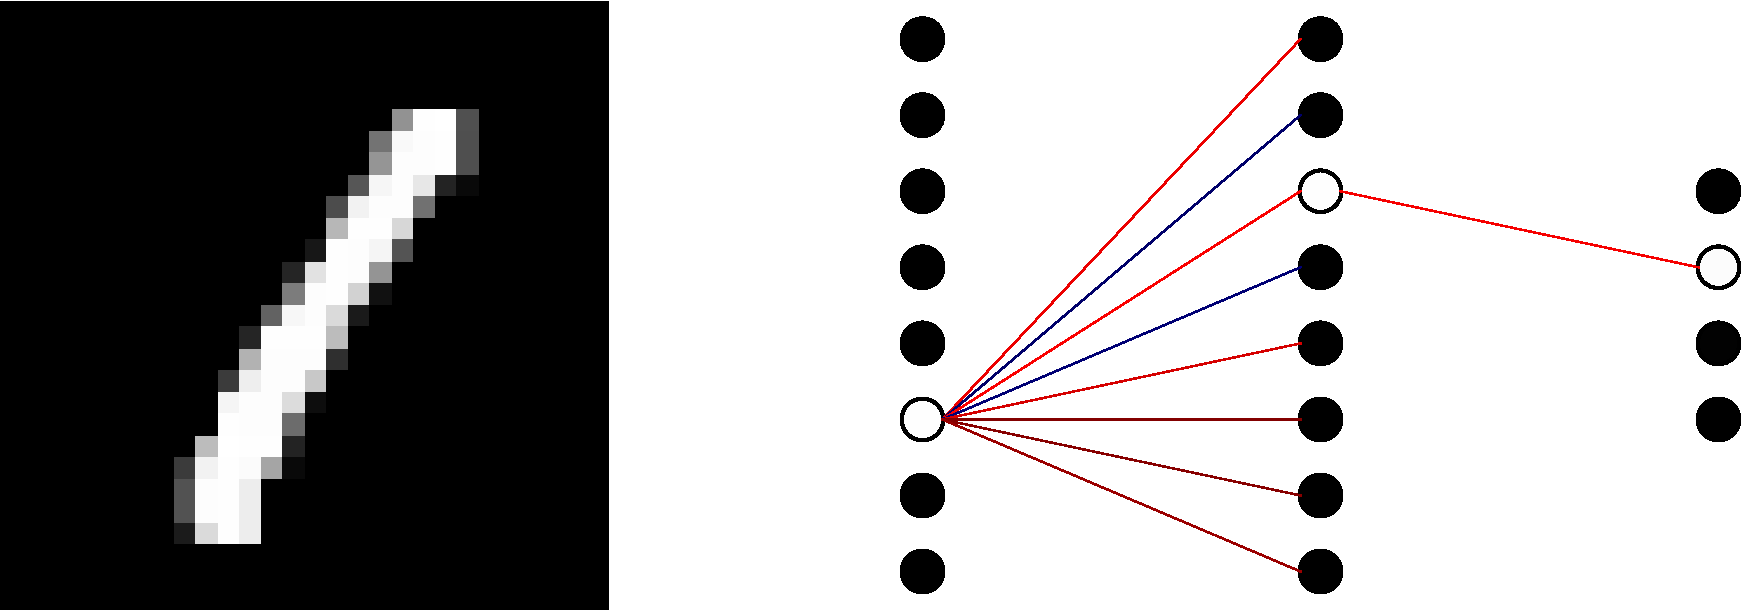
\includegraphics[width=0.9\textwidth]{figures/backpropimg13.pdf}
		\end{figure}
	\end{columns}
	\vfill
	$$
		x_3^2 = \sigma_3\left(A_{3}^{2,1}x_2^1+A_{3}^{2,2}x_2^2 +\dots+A_{3}^{2,8}x_2^8\right)
	$$
\end{frame}


\subsection{Example : Image classification of handwritten digits from A to Z}

\begin{frame}
	Having discussed the theory behind Artificial Neural Networks and the training process, we will now proceed to demonstrate a comprehensive end-to-end example of image classification on MNIST.
	\vskip 0.5cm
	\begin{figure}
		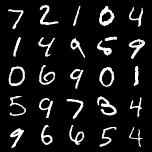
\includegraphics[width=0.4\textwidth]{figures/MNIST_full_dense.png}
	\end{figure}
\end{frame}

\begin{frame}
	\begin{itemize}
		\item Input shape : $1 \times 28 \times28$.
		\item Number of Classes : $10$.
		\item Number of training samples $(x, y)$: $60000$.
		\item Number of evaluating samples: $10000$.
		\item Loss : cross-entropy
		      $$L(\hat{y}, y) = - \frac{1}{N} \sum_{i=1}^{N} \sum_{j=1}^{K} y_{ij} \log(\hat{y}_{ij})$$
		      where :
		      \begin{itemize}
			      \item $\hat{y} \in \mathbb{R}^{N \times K}$ is the predicted probability distribution over $K$ classes for $N$ samples,
			      \item $y \in {0,1}^{N \times K}$ is the ground-truth one-hot encoded label matrix,
		      \end{itemize}
	\end{itemize}
\end{frame}

\begin{frame}{Recap on the Cross-Entropy Loss}

	\begin{tikzpicture}
		% One-hot distribution
		\begin{axis}[
				title={One-Hot Distribution ($y_i$)},
				height=6cm, width=9cm,
				symbolic x coords={Class 1, Class 2, Class 3, Class 4, Class 5},
				xtick=data,
				ymin=0, ymax=1,
				ytick={0, 0.2, 0.4, 0.6, 0.8, 1},
				bar width=0.6cm,
				nodes near coords,
				enlarge x limits=0.3,
				grid=major,
				ticklabel style={font=\footnotesize}
			]
			\addplot[ybar,fill=primary] coordinates {
					(Class 1, 0)
					(Class 2, 0)
					(Class 3, 1)
					(Class 4, 0)
					(Class 5, 0)
				};
		\end{axis}
	\end{tikzpicture}
	\hfill
	\begin{tikzpicture}
		% Model predicted distribution
		\begin{axis}[
				title={Model Predicted Distribution ($\hat{y}_i$)},
				height=6cm, width=9cm,
				symbolic x coords={Class 1, Class 2, Class 3, Class 4, Class 5},
				xtick=data,
				ymin=0, ymax=1,
				ytick={0, 0.2, 0.4, 0.6, 0.8, 1},
				bar width=0.6cm,
				nodes near coords,
				enlarge x limits=0.3,
				grid=major,
				ticklabel style={font=\footnotesize}
			]
			\addplot[ybar,fill=secondary] coordinates {
					(Class 1, 0.1)
					(Class 2, 0.15)
					(Class 3, 0.5)
					(Class 4, 0.2)
					(Class 5, 0.05)
				};
		\end{axis}
	\end{tikzpicture}

	The cross-entropy loss for one sample is:
	$$
		l(\hat{y}_i, y_i) = -  \sum_{j=1}^{K} y_{ij} \log(\hat{y}_{ij}).
	$$

\end{frame}

\begin{frame}
	We build a 3 layers network.
	\begin{itemize}
		\item Batch size : 64
		\item Learning rate : 0.01
		\item Intermediate activation : ReLU
		\item Final activation : Softmax
		\item Number of epochs : 12
		      % \item Scheduler : we divide $\lambda$ by $2$ every 3 epochs.
		\item Number of trained parameters: $52.6$k
	\end{itemize}

	\begin{figure}
		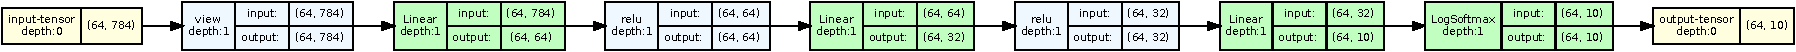
\includegraphics[width=\textwidth]{figures/densemnist.pdf}
	\end{figure}
\end{frame}
\begin{frame}
	\begin{figure}
		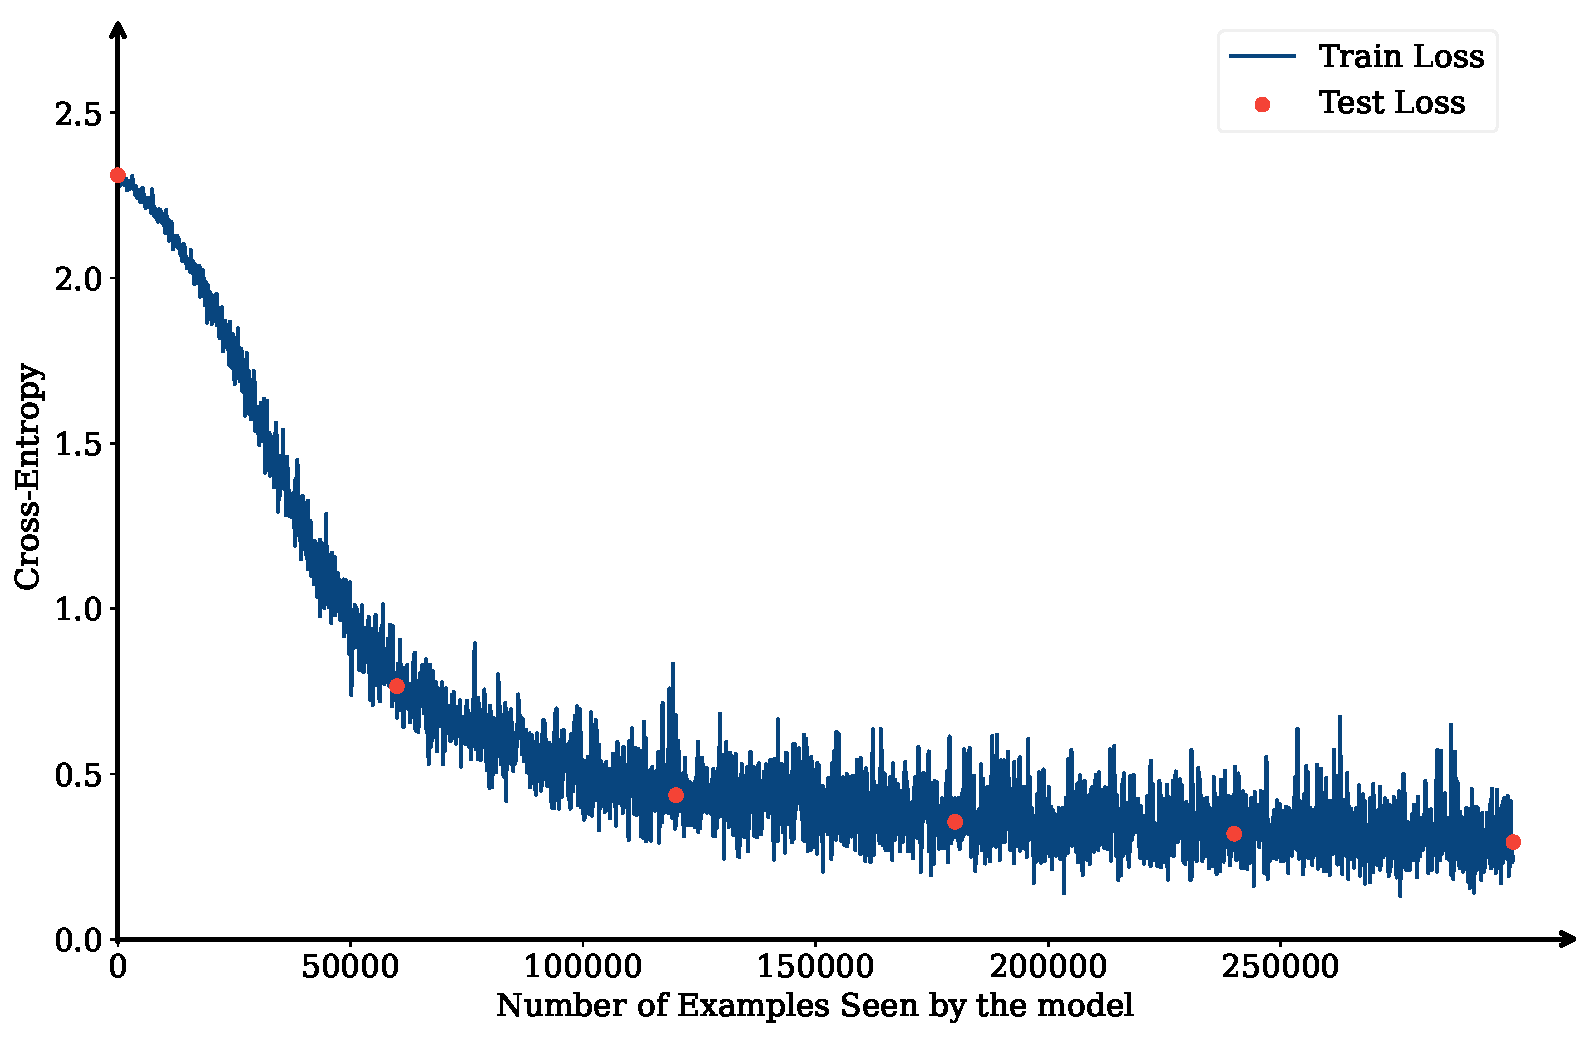
\includegraphics[width=0.7\textwidth]{figures/densemnist_res.pdf}
	\end{figure}
\end{frame}
% \begin{frame}
% 	With an interpretation tool such as SHAP:
% 	\begin{figure}
% 		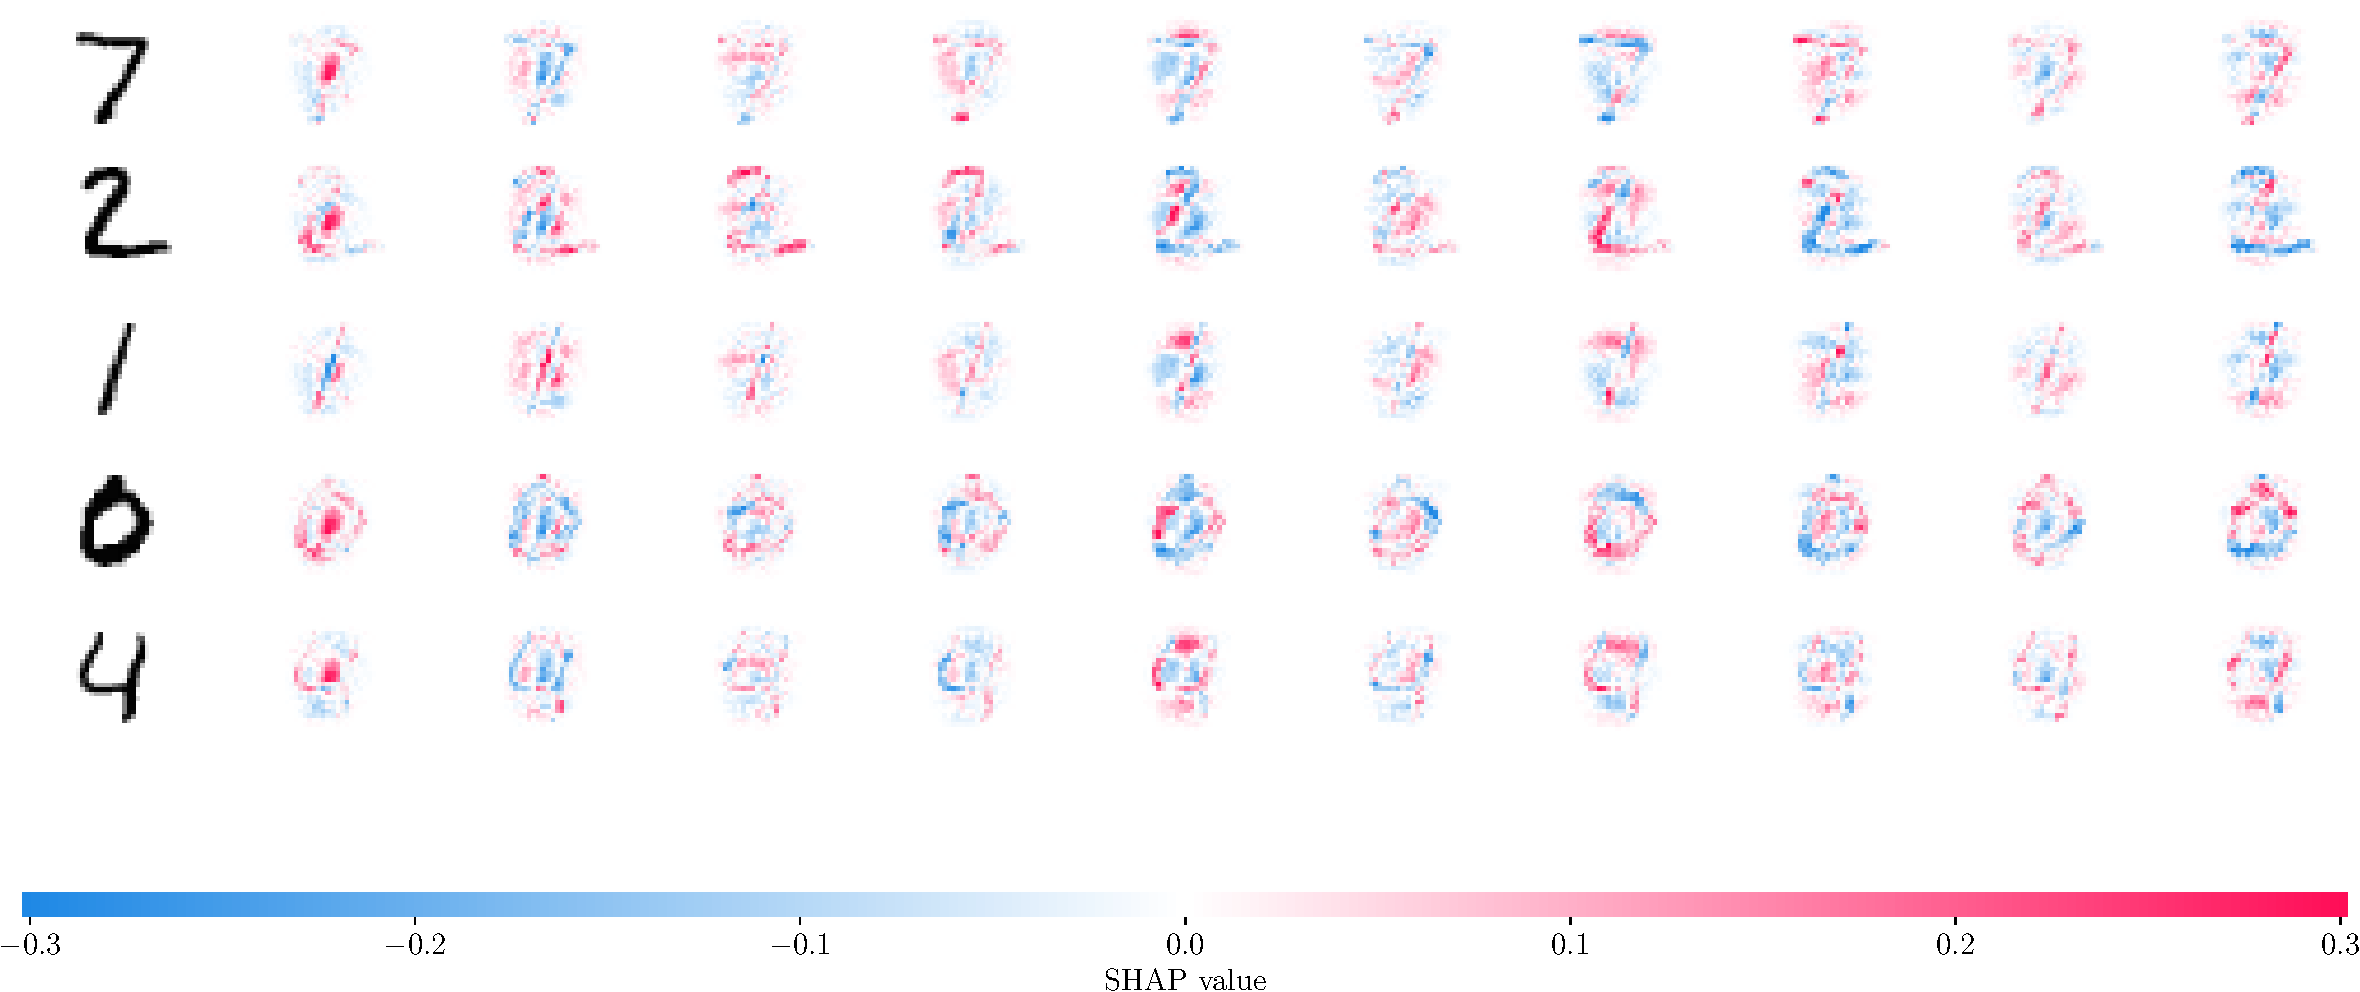
\includegraphics[width=1\textwidth]{figures/shapdense.pdf}
% 	\end{figure}
% \end{frame}

\begin{frame}{The Multi-layer Perceptron (MLP)}{The first Deep Learning Model}
	Link to the notebook: \href{
		https://lamsade.dauphine.fr/~averine/EM_IASD/TP1.ipynb}{Notebook Collab}\\
	Link to the notebook: \href{https://lamsade.dauphine.fr/~averine/EM_IASD/TP1.html}{html}
\end{frame}

\begin{frame}{}{Your turn !}
	Get the Notebook on the course website and start working on it.
	\begin{itemize}
		\item \url{https://www.alexverine.com}
		\item Teaching
		\item Introduction to Deep Learning
		\item Lien Notebook
	\end{itemize}
	During this hands-on session we get you started with the basics of deep learning using PyTorch. You will implement a simple feedforward neural network (Multi-Layer Perceptron) to classify handwritten digits from the MNIST dataset.
\end{frame}
